
%%%%%%%%%%%%%%%%%%%%%%%%%%%%%%%%%%%%%%%%%%%%%%%%%%%%%%%%%%%%%%%
%%%%%%%%%%%%%%%%% AIRFOIL OPTIMIZATION %%%%%%%%%%%%%%%%%%%%%%%%
%%%%%%%%%%%%%%%%%%%%%%%%%%%%%%%%%%%%%%%%%%%%%%%%%%%%%%%%%%%%%%%

\section{Airfoil Design}
\label{airfoil}

In this section the robust optimization of an airfoil is discussed.

\subsection{Aerodynamic Analysis}
The steady inviscid flow around an airfoil governed by the Euler equations is solved by using a second-order accurate finite-volume approach~\cite{Mani2007a,Mani2007b}.
The computational mesh is shown in Figure~\ref{fig:mesh}.
Hicks-Henne sine bump functions~\cite{Hicks78} are used to control the shape of the airfoil resulting from perturbations of shape design variables.
The resulting deformation of the mesh is calculated via a linear tension spring analogy~\cite{Batina90,Mani2008a}.

\begin{figure}[h]
  \centering  
  \begin{minipage}[b]{0.45\linewidth}
    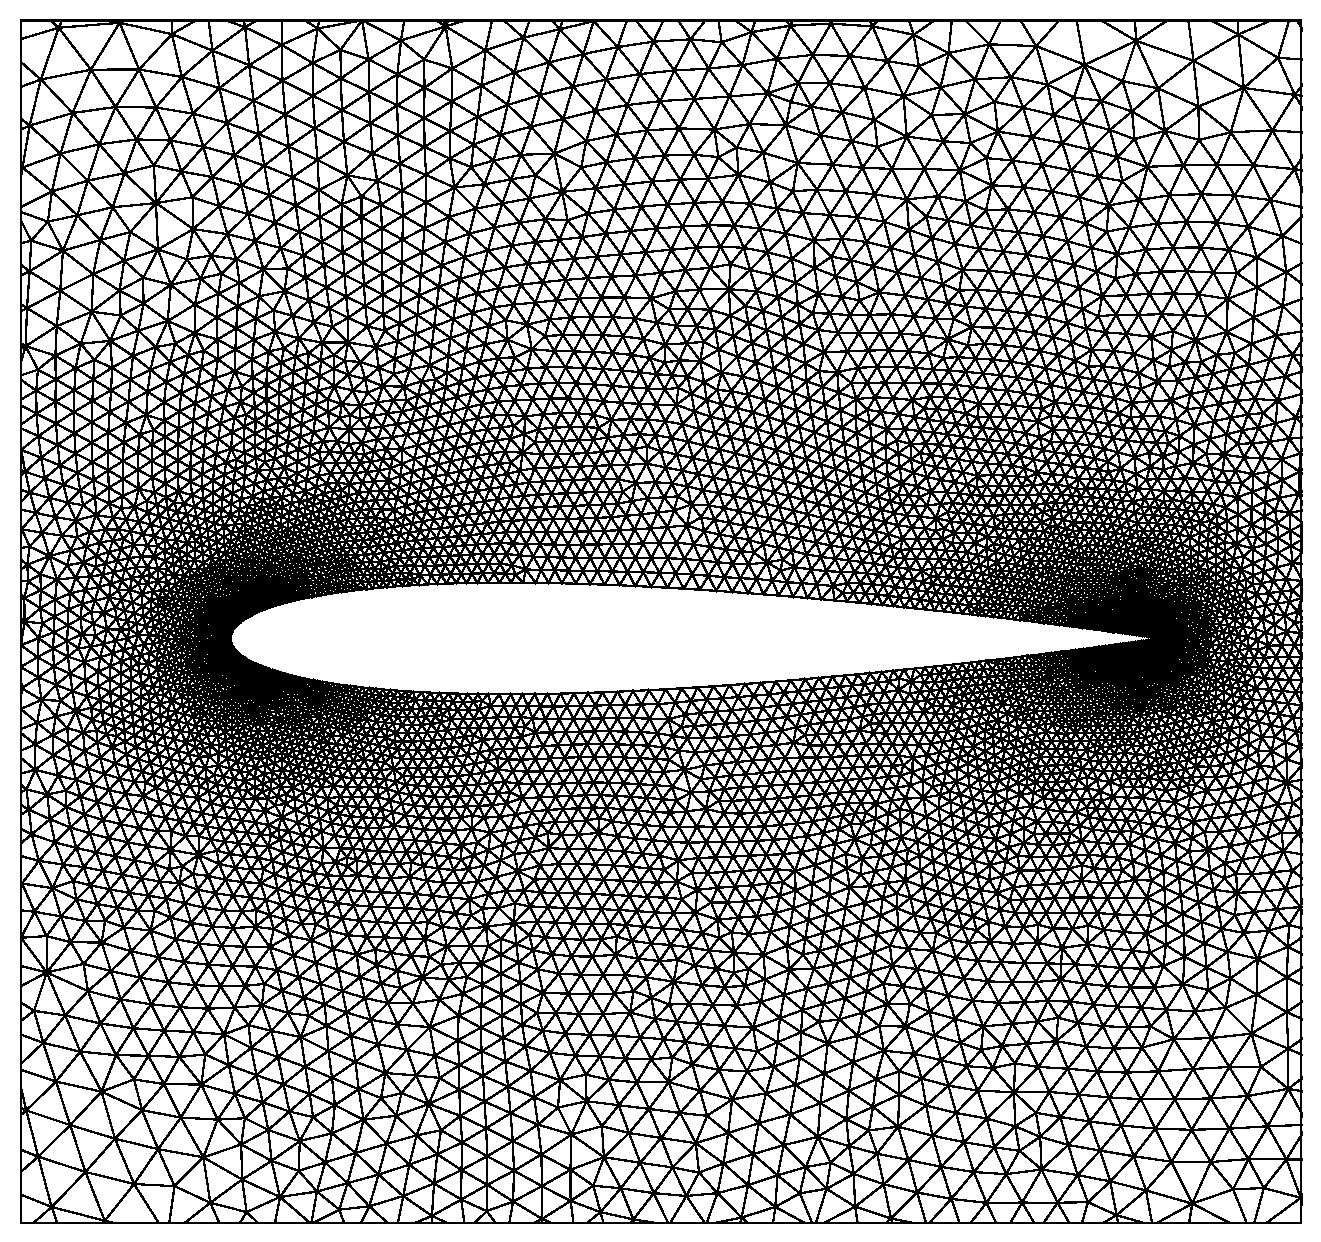
\includegraphics[width=1.0\textwidth]{finemesh.eps} 
  \end{minipage}
  \begin{minipage}[b]{0.475\linewidth}
    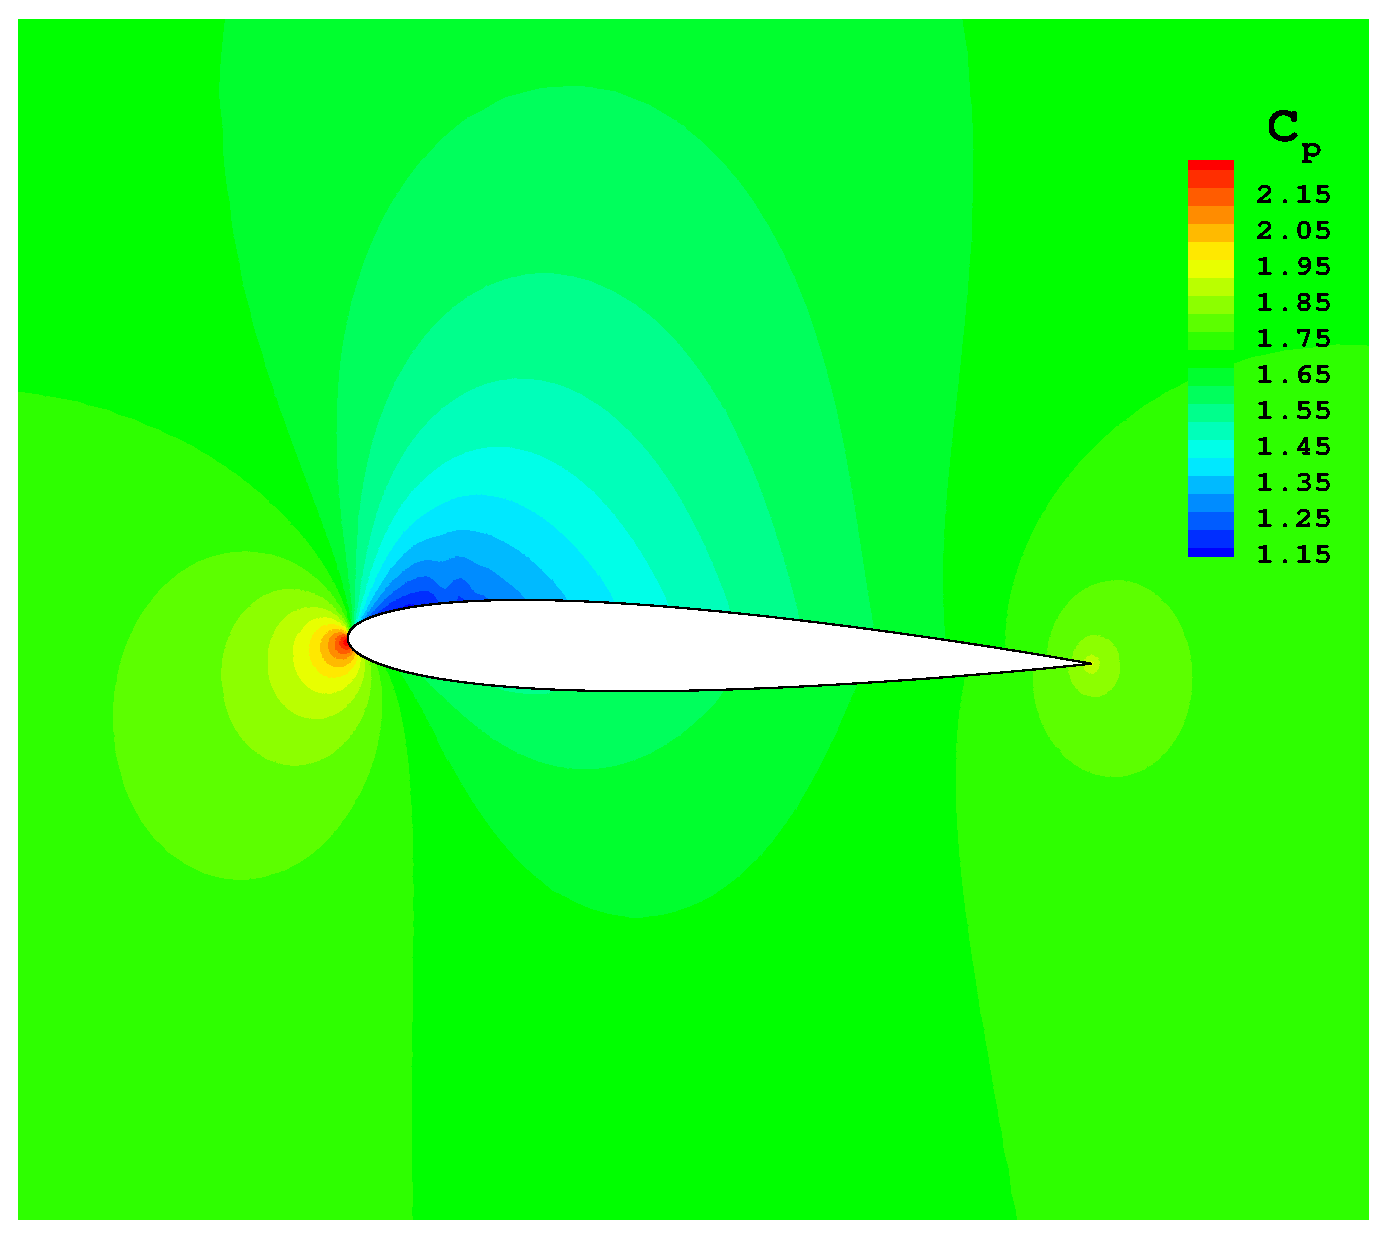
\includegraphics[width=1.0\textwidth]{cpcontouralpha2mach65.eps} 
  \end{minipage}
  \caption[Computational mesh for NACA 0012.]{Computational mesh for NACA 0012 airfoil with $19,548$ elements (left), pressure distribution at $\alpha=2.0^\circ$ and M=0.65 (right).}
  \label{fig:mesh}
\end{figure}



\subsection{Robust Optimization Problem}
Seven shape design variables are placed on the upper surface and seven on the lower surface of the airfoil (at 20\%, 30\%, 40\%, 50\%, 60\%,  80\%, and 90\% chord). 
The bounds on the flow variables, angle of attack and Mach number, are taken as $0^\circ \le \alpha \le 4^\circ$ and $0.6 \le  M \le 0.78$.
\begin{figure}[h]
\centering
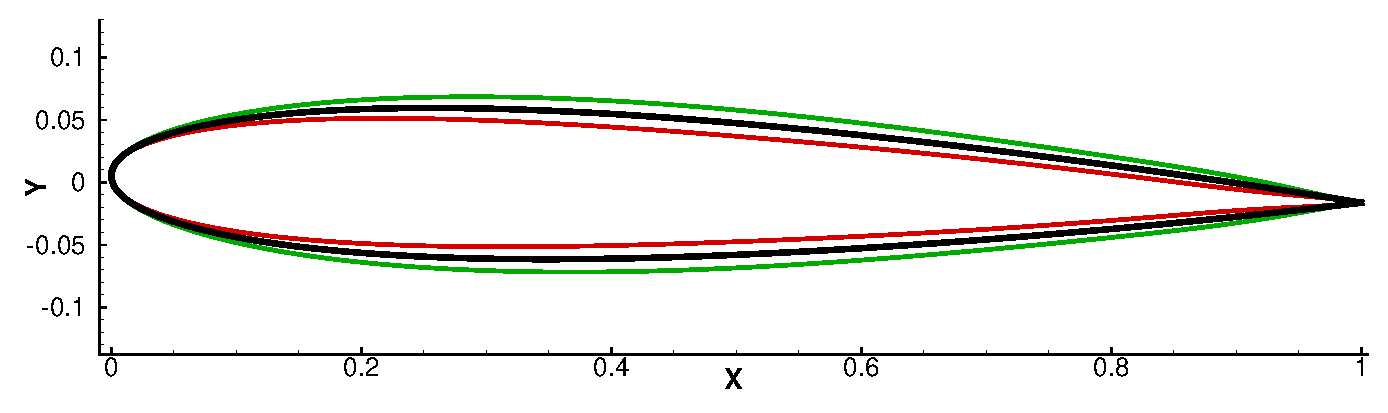
\includegraphics[width=0.8\textwidth]{Uncertainshapes14DV.eps}
\caption[NACA 0012 airfoil with shape perturbations.]{The NACA 0012 airfoil (in black) and airfoils resulting from perturbations of \mbox{$\pm 0.0025$} (in red and blue).} \label{Uncertainshapes14DV}
\end{figure}
All fourteen shape design variables are assumed to have epistemic uncertainties and the two flow variables are assumed to have aleatory uncertainties.

\begin{table}[h!]
  \caption{Data for robust optimization of airfoil.}
  \medskip
  \centering 
  \begin{tabular}{cccccc}
    \hline\hline
   Random   & Description    & Uncertainty        & $\tau_{min}$  & $\tau_{max}$             & Standard    \\
   Variable & & Type         &    &                &   Deviation  \\
    \hline\hline
    $\ns_{1,2,13,14}$   & Shape design variables  & Epistemic      & -0.00125 & 0.00125  &  -      \\
    $\ns_{3-12}$       & Shape design variables & Epistemic     & -0.01    &   0.01   &   -       \\
\hline
    $\xi_\alpha$        & Angle of attack  & Aleatory           &    -        & -   &  $0.1^\circ$  \\
    $\xi_M$            &  Mach number  & Aleatory              &    -          &   -   &  0.01    \\
    \hline
  \end{tabular}
  \label{tab:rv_data_cfd14}
\end{table}
Figure~\ref{Uncertainshapes14DV} shows the baseline NACA 0012 airfoil used as the initial (starting) design and the airfoils resulting from perturbations of the fourteen shape design variables within the bounds specified in Table~\ref{tab:rv_data_cfd14}.  
The initial value of the angle of attack is $2^\circ$ and the Mach number is $0.65$.
The mathematical formulation of the problem is given as follows,
\beq \label{eq:cfdrob}
\begin{aligned}
& \underset{\z,\n}{\text{minimize}}
& & {\J}=\mu_{{C}_{d_{max}}}+{\sigma_{C_{d_{max}}}^2}, \\
& \text{subject to}
  & & g =(\mu_{{C}_{l_{min}}}+k{\sigma_{C_{l_{min}}}})-{C_l}^{+} \geq 0,
\end{aligned}
\eeq
\noindent where $C_l^{+}$ refers to a target lift coefficient of $0.6$, and $C_{l_{min}}$ and $C_{d_{max}}$ are the least possible lift and highest possible drag within the specified set of epistemic variables, respectively. 

\paragraph{Surrogate models:}The kriging surrogate model is built with 11 training points. The polynomial chaos surrogate is a second-order polynomial with an over sampling factor of two forming a regression surface which requires 12 training points. 
The surrogate models are built only over the assumed aleatory variables: the angle of attack and Mach number. The domain of the surrogate model is three standard deviations wide from the mean values $\bar{\z}$ provided by the main optimizer (IPOPT) at every iteration.

\subsection{Optimization Results}
\begin{table}[h!]
\caption{Optimization results for airfoil design problem.}
\medskip
\centering 
\scalebox{0.78}{\begin{tabular}{c|cc|cc|cc|cc|c}
\hline\hline
Type  & k  & $P_k$ & $\mu_{{c}_{d_{max}}}$ & ${\sigma_{c_{d_{max}}}^2}$ & $\mu_{{c}_{l_{min}}}$ &  ${\sigma_{c_{l_{min}}}}$ & $\alpha$ & $M$ & No. of F/FG Evals.\\
& & & & & & & & & $\&$ Iterations\\
\hline\hline
Initial        & - & - & $4.72\cdot 10^{-4}$ & - & 0.335  & - & $2.000^\circ$ & 0.650 &\\
\hline
Deterministic  & - & - & $1.17\cdot 10^{-3}$ & - & 0.600  & - & $2.510^\circ$ & 0.600 & 49/49-24 \\
\hline
Robust-KR & 0  & 0.5000 & $2.72\cdot 10^{-3}$ & $2.03\cdot 10^{-7}$ & $0.600$ & $1.84\cdot 10^{-2}$ & $2.013^\circ$ & 0.600 & 844/844-23 \\
Robust-PC      & 0  & 0.5000 & $2.62\cdot 10^{-3}$ & $5.80\cdot 10^{-8}$ & $0.600$ & $1.82\cdot 10^{-2}$ & $2.389^\circ$ & 0.600 & 675/6751-16\\
\hline
Robust-KR & 1  & 0.8413 & $2.93\cdot 10^{-3}$ & $3.07\cdot 10^{-7}$ & $0.619$ & $1.86\cdot 10^{-2}$ & $2.065^\circ$ & 0.600 & 434/434-13\\ 
Robust-PC      & 1  & 0.8413 & $2.73\cdot 10^{-3}$ & $2.50\cdot 10^{-7}$ & $0.618$ & $1.84\cdot 10^{-2}$ & $3.058^\circ$ & 0.600 & 434/434-15 \\
\hline
Robust-KR & 2  & 0.9772 & $3.10\cdot 10^{-3}$ & $4.46\cdot 10^{-7}$ & $0.637$ & $1.88\cdot 10^{-2}$ & $2.179^\circ$ & 0.600 & 831/831-19\\ 
Robust-PC      & 2  & 0.9772 & $3.20\cdot 10^{-3}$ & $8.58\cdot 10^{-7}$ & $0.637$ & $1.89\cdot 10^{-2}$ & $2.193^\circ$ & 0.600 & 710/710-22\\ 
\hline
Robust-KR & 3  & 0.9986 &$3.28\cdot 10^{-3}$ & $6.23\cdot 10^{-7}$ & $0.657$ & $1.90\cdot 10^{-2}$ & $2.301^\circ$ & 0.600 & 650/650-21\\
Robust-PC      & 3  & 0.9986 &$3.25\cdot 10^{-3}$ & $9.83\cdot 10^{-7}$ & $0.658$ & $1.92\cdot 10^{-2}$ & $2.352^\circ$ & 0.600 & 1145/1145-21\\
\hline
Robust-KR & 4  & 0.9999 &$3.56\cdot 10^{-3}$ & $9.50\cdot 10^{-7}$ & $0.677$ & $1.93\cdot 10^{-2}$ & $2.421^\circ$ & 0.600 & 620/620-15\\
Robust-PC      & 4  & 0.9999 &$3.65\cdot 10^{-3}$ & $1.25\cdot 10^{-6}$ & $0.677$ & $1.93\cdot 10^{-2}$ & $2.427^\circ$ & 0.600 & 2104/2104-36\\
\hline
\end{tabular}}
\label{tab:CFD14results}
\end{table}
Table~\ref{tab:CFD14results} compares the robust design optima with the deterministic optimum.  %It can be seen that the deterministic $\alpha^*$ is the highest of all, i.e. deterministic optimization achieves the target lift predominantly by increasing the angle of attack, rather than changing the airfoil shape. 
The average drag and mean angle of attack increase as the desired probability of achieving the target lift $C_l^{+}$  is increased. 
The optimum solution is sought from the optimizer at a distance of $k$-standard deviations away from the lift-constraint hyperplane.
As a result, the amount of lift produced is higher as more robustness is expected from the design \ie~the additional lift produced defines the robustness of the design and the design will be less prone to failure (violation of the lift-constraint).
On the contrary, during a deterministic optimization an optimum design is sought at the constraint boundary, that can very well violate design requirements when the underlying variables are not representative of the ones considered during optimization. Another inference is that robustness is achieved at the expense of the objective function (drag penalty).
Also by observing the optimum aleatory variables on the right, it can be seen that the Mach number remains the same for all designs (at its lower bound), 
whereas the angle of attack varies.





\subsubsection{Airfoil shape}

Figure~\ref{airfoils} shows the original, deterministic and robustly optimized ($k=4$, with polynomial chaos) airfoils. It can be inferred that the deterministically optimized airfoil (shown in blue) looks very thin compared to the robustly optimized airfoil (shown in red). %The deterministic designs lower shape design variables take same values as that of the robust one. 

%\paragraph{Deterministic versus robust airfoils:}

\begin{figure}[H]
  \centering  
%  \begin{minipage}[b]{0.45\linewidth}
 %   \includegraphics[width=1.0\textwidth]{OptshapesKrig.eps} 
% \end{minipage}
  \begin{minipage}[b]{0.90\linewidth}
    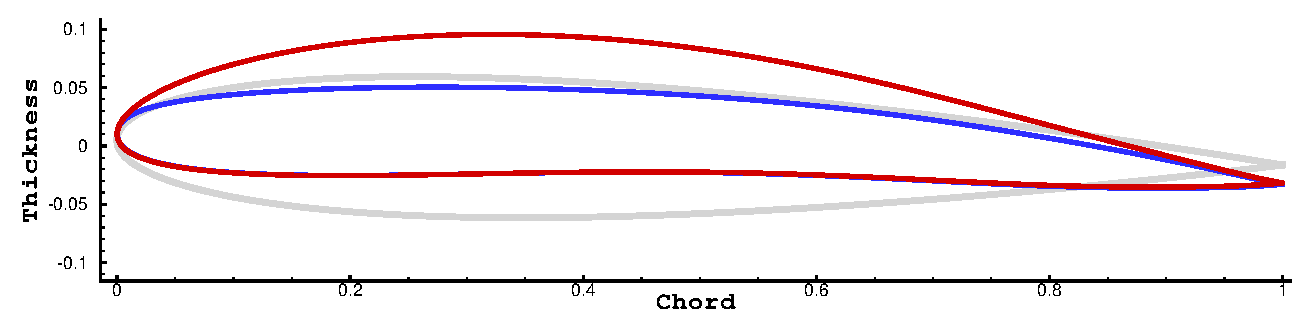
\includegraphics[width=1.0\textwidth]{OptshapesPC.eps} 
  \end{minipage}
  \caption[Shapes of the initial, deterministic and robust airfoils.]{Original NACA 0012 (gray), deterministic (blue) and robust with $k=4$ (red) airfoils produced using polynomial chaos. The kriging produced very similar airfoils (hence not shown).}
  \label{airfoils}
\end{figure}


\begin{figure}[H]
  \centering  
  \begin{minipage}[b]{0.90\linewidth}
    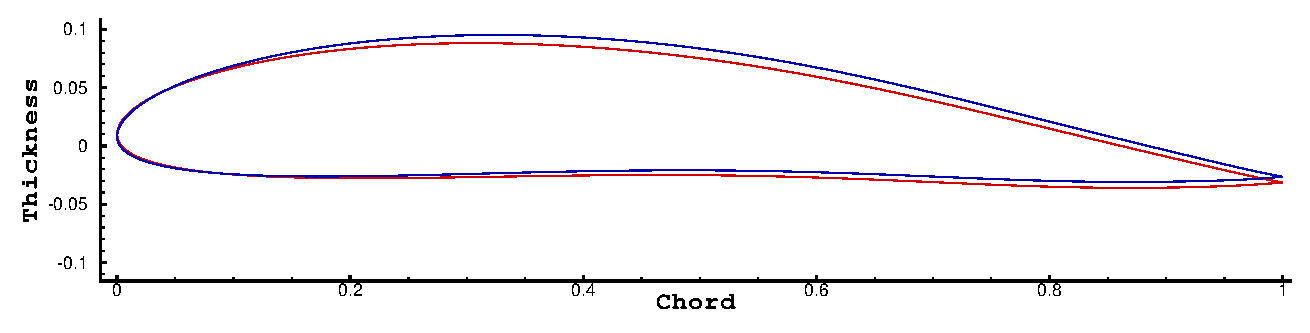
\includegraphics[width=1.0\textwidth]{Shapesk0.eps} \subcaption{Robust Airfoils $k=0$}
  \end{minipage}
  \begin{minipage}[b]{0.90\linewidth}
    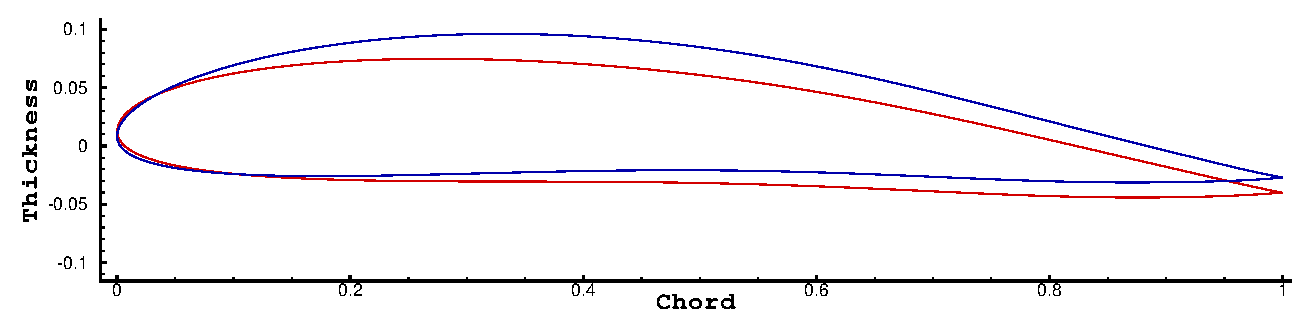
\includegraphics[width=1.0\textwidth]{Shapesk1.eps} \subcaption{Robust Airfoils $k=1$}
  \end{minipage}
  \begin{minipage}[b]{0.90\linewidth}
    \includegraphics[width=1.0\textwidth]{Shapesk2.eps} \subcaption{Robust Airfoils $k=2$}
  \end{minipage}
  \begin{minipage}[b]{0.90\linewidth}
    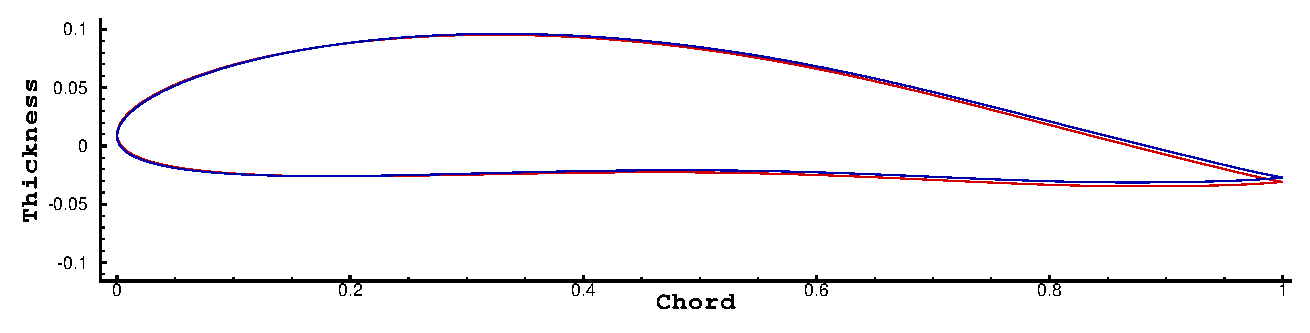
\includegraphics[width=1.0\textwidth]{Shapesk3.eps} \subcaption{Robust Airfoils $k=3$}
  \end{minipage}
  \begin{minipage}[b]{0.90\linewidth}
    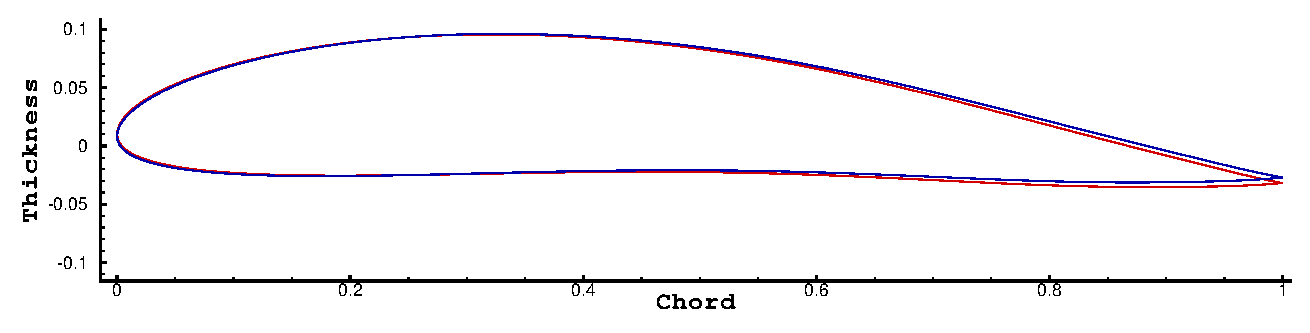
\includegraphics[width=1.0\textwidth]{Shapesk4.eps} \subcaption{Robust Airfoils $k=4$}
  \end{minipage}
  \caption[Shapes of different robust airfoils.]{Plots showing the shape (also angle of attack) of different robust airfoils. Red and blue lines correspond to polynomial chaos and kriging, respectively.}
  \label{robustairfoils}
\end{figure}

The robust airfoils corresponding to increasing $k$ are shown in Figure~\ref{robustairfoils}. Except for the first two cases ($k=0$ and $k=1)$, the epistemic shape design variables attain similar values for both models. 
For $k=1$ case, the kriging based robust airfoil is thicker and has a lower angle of attack, whereas the polynomial chaos based airfoil is thinner and attains the target lift with an increased angle of attack.


%\paragraph{Comparison within robust airfoils:}
Overall, the kriging surrogate based robust designs (shown as blue lines) tend to have a lower angle of attack than its polynomial chaos counterpart (shown as red line). This behavior can be observed across all five robust designs. 
In general, it may be advantageous for an airplane to fly faster rather than having an increased angle of attack for generating more lift. The solution to the Euler equations ignores important viscous effects, such as boundary layers, wakes and flow separation. 
If a Navier-Stokes solver is used, it can be expected that the optimizer places a greater emphasis on the shape optimization rather than the flow parameter optimization.

%\begin{figure}[h!]
%  \centering
%  \begin{minipage}[b]{0.47\linewidth}
%    \includegraphics[width=1.0\textwidth]{cpdet14dv.eps} 
%  \end{minipage}
%  \b
%    \includegraphics[width=1.0\textwidth]{rob14dvk2krg.eps} 
%  \end{minipage}
%  \begin{minipage}[b]{0.47\linewidth}
%    \includegraphics[width=1.0\textwidth]{cprob14dvk2pc.eps} 
%  \end{minipage}
%  \caption{Plots of pressure distributions at optimum designs (left: deterministic, right: robust with PC).}
%  \label{optcpcontours}
%\end{figure} 

\subsubsection{Simulation Requirements}

The last column of Table~\ref{tab:CFD14results} presents the number of function and gradient evaluations needed as well as the number of iterations taken by the optimizer to converge. Here a single flow solve provides the lift (constraint) and drag (objective) values. 
For this airfoil optimization test case, the robust optimization needs on average roughly $1000$ flow and adjoint solutions, compared to close to $50$ evaluations needed for the deterministic optimization, placing a roughly 20 times higher simulation requirement on the designer. The box-constrained optimizations took 2 to 3 flow and adjoint solutions to determine the worst possible lift and the highest possible drag within the specified epistemic uncertainty bounds. For the aleatory uncertainty propagation, though kriging and polynomial chaos involve the same amount of training information (eleven and twelve points respectively), at the end of the main optimization, the latter's simulation requirements are $50\%$ higher than that of the kriging (on average). 
This shows that kriging is more effective for non-smooth functions such as this aerodynamic test case.

\begin{figure}[h]
  \centering  
  \begin{minipage}[b]{0.9\linewidth}
    \includegraphics[width=1.0\textwidth]{cfditerhist.eps} 
  \end{minipage}
  \caption[Optimization history for airfoil design problem.]{Optimizer iteration history for airfoil design problem.}
  \label{CFDIterHist}
\end{figure}

Figure~\ref{CFDIterHist} plots the change in the objective function with the number of optimizer iterations. 
\subsubsection{Output PDF and CDF at the Optimum}
\begin{figure}[h]
  \centering  
  \begin{minipage}[b]{0.47\linewidth}
    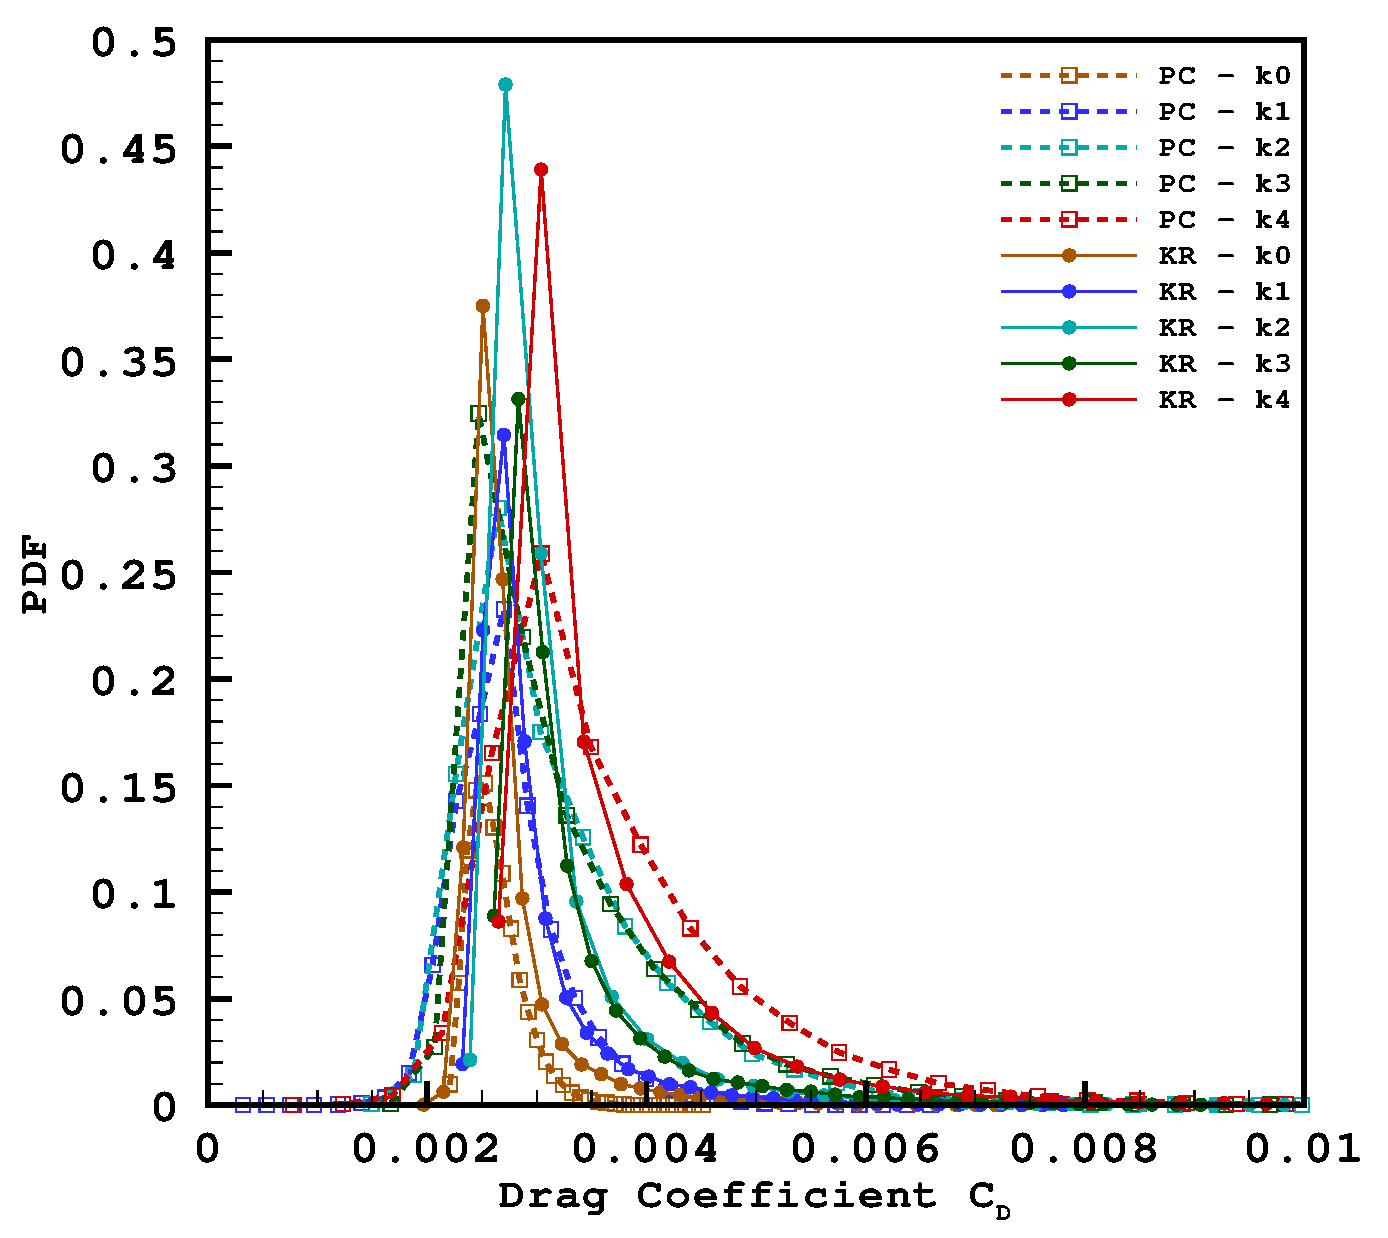
\includegraphics[width=1.0\textwidth]{cfdpdfallcon0.eps} 
  \end{minipage}
  \begin{minipage}[b]{0.47\linewidth}
    \includegraphics[width=1.0\textwidth]{cfdcdfallcon0.eps} 
  \end{minipage}
  \caption{PDF and CDF of the drag coefficient at optimum designs.}
  \label{CFDDrag}
\end{figure}
 Figures~\ref{CFDDrag} and~\ref{CFDLift} show the PDF as well as CDF of the drag and lift coefficients, respectively, at several robust designs using kriging and polynomial chaos. The PDFs shown in the left shows the distribution of possible drag and lift coefficient values due to the effect of uncertainties, whereas the CDFs show the probability of obtaining a specified value or less. For example, the distribution of drag (see the left of Figure~\ref{CFDDrag}) helps the designer to construct confidence bounds on possible drag values. Similarly, the probability that the target lift coefficient ($C_L^+=0.6$) is not attained is $50\%$ for the $k=0$ case and is less than $1\%$ for the $k=4$ case. As the required robustness increases, the distributions shift to the right, which signifies a higher lift generation as well as drag penalty. A Gaussian distribution is seen for the lift coefficient, whereas  the distribution of drag coefficient resembles a log-normal one. 
\begin{figure}[h]
  \centering  
  \begin{minipage}[b]{0.47\linewidth}
    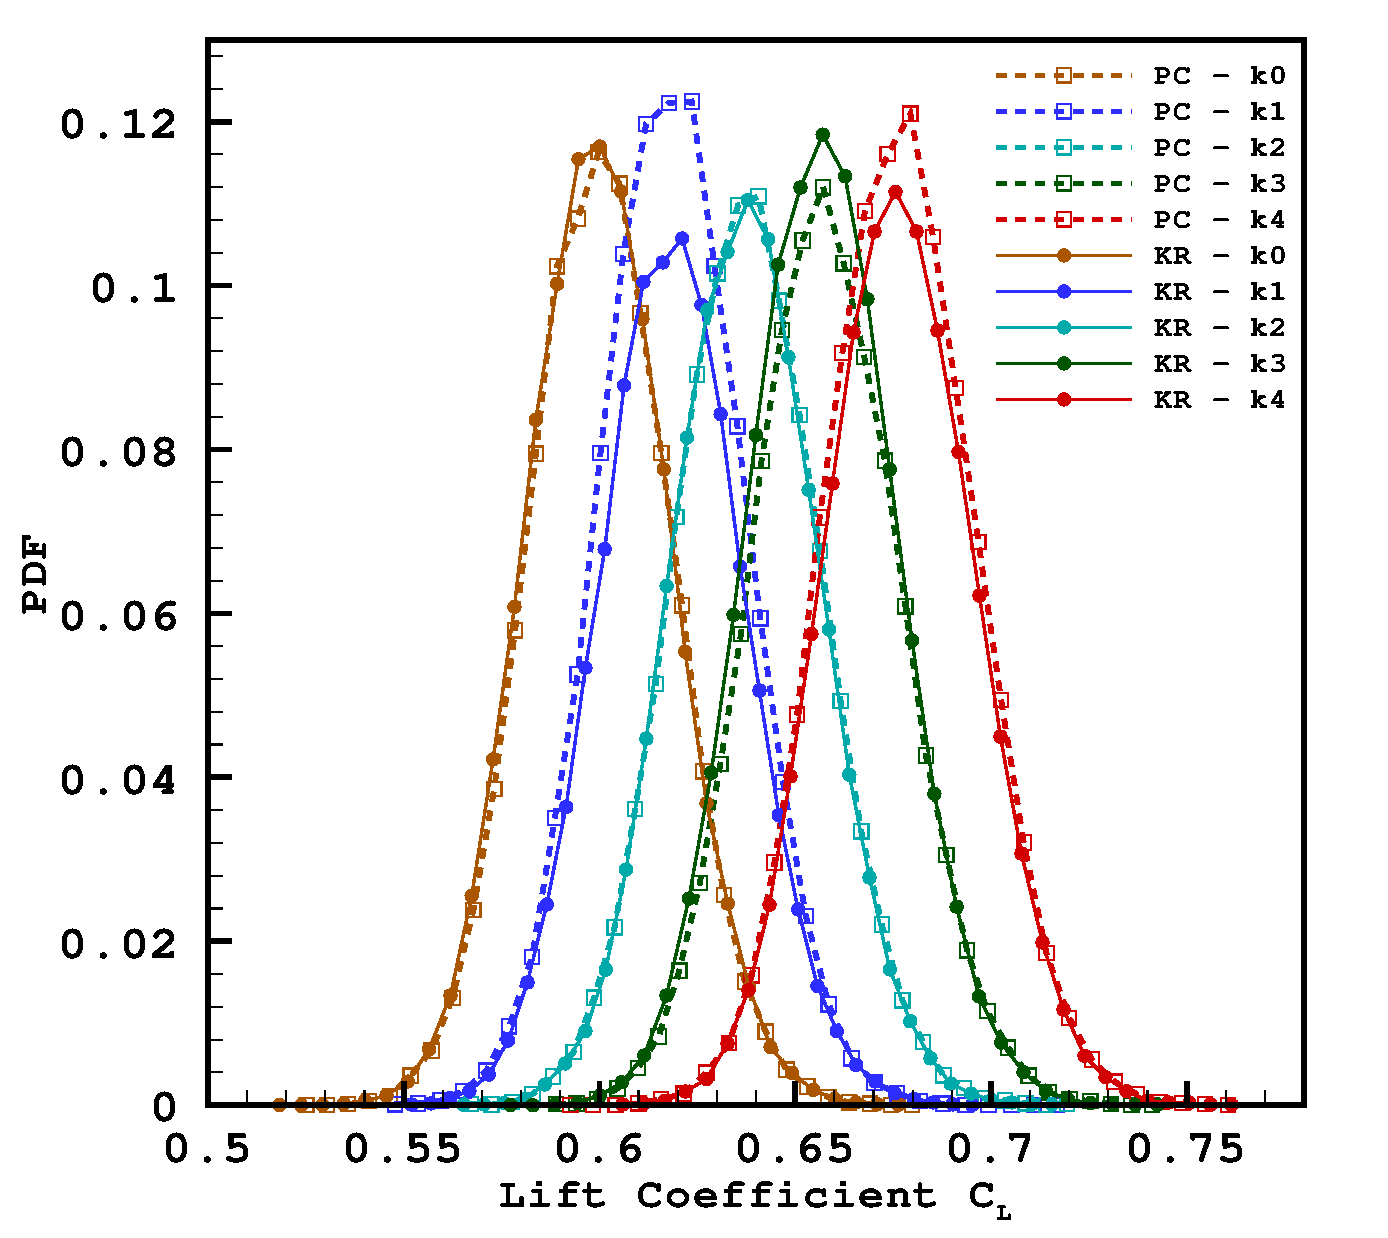
\includegraphics[width=1.0\textwidth]{cfdpdfallcon1.eps} 
  \end{minipage}
  \begin{minipage}[b]{0.47\linewidth}
    \includegraphics[width=1.0\textwidth]{cfdcdfallcon1.eps} 
  \end{minipage}
  \caption{PDF and CDF of the lift coefficient at optimum designs.}
  \label{CFDLift}
\end{figure}



\subsubsection{Pressure Contours at the Optimum}
Figures~\ref{CpContoursRobustKriging} and ~\ref{CpContoursRobustPC} show the pressure distribution around deterministically and robustly optimized airfoils using kriging and polynomial chaos, respectively. 
It can be seen that the pressure distributions are very similar among the robust airfoils, whereas a distinct difference can be noticed between the robust and deterministic ones.
\begin{figure}[h]
  \centering  
  \begin{minipage}[b]{0.30\linewidth}
    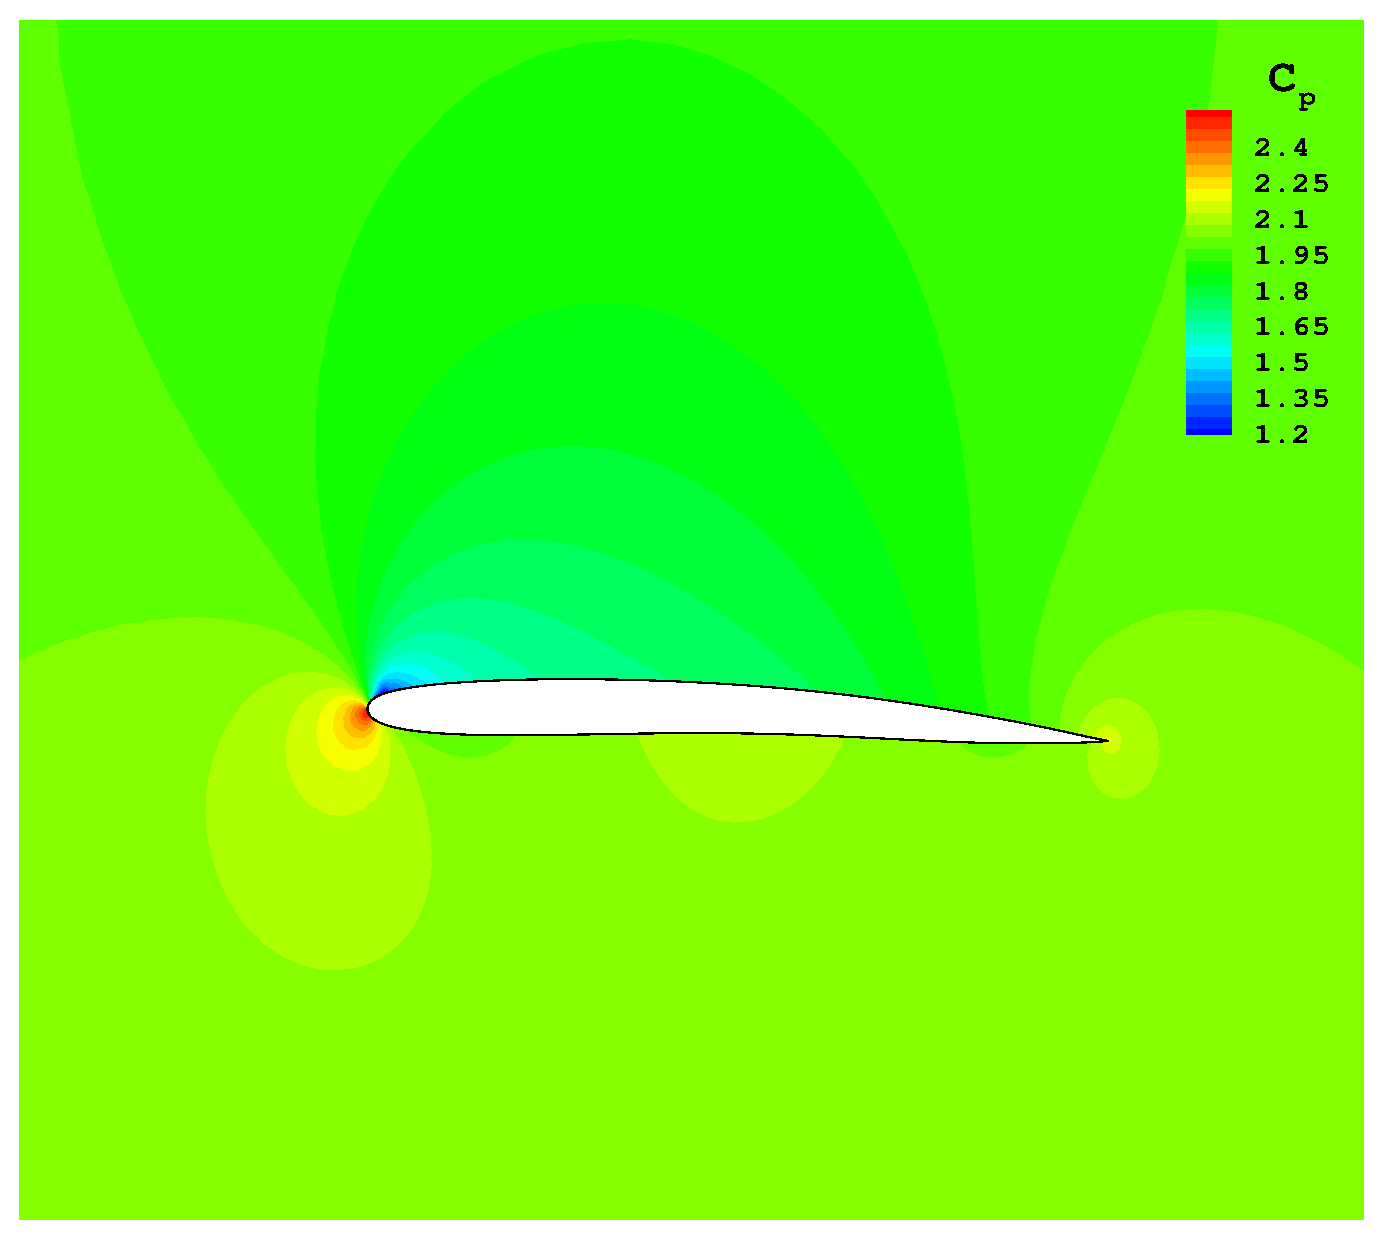
\includegraphics[width=1.0\textwidth]{DeterministicPressure.eps} \subcaption{Deterministic}
  \end{minipage}
  \begin{minipage}[b]{0.30\linewidth}
    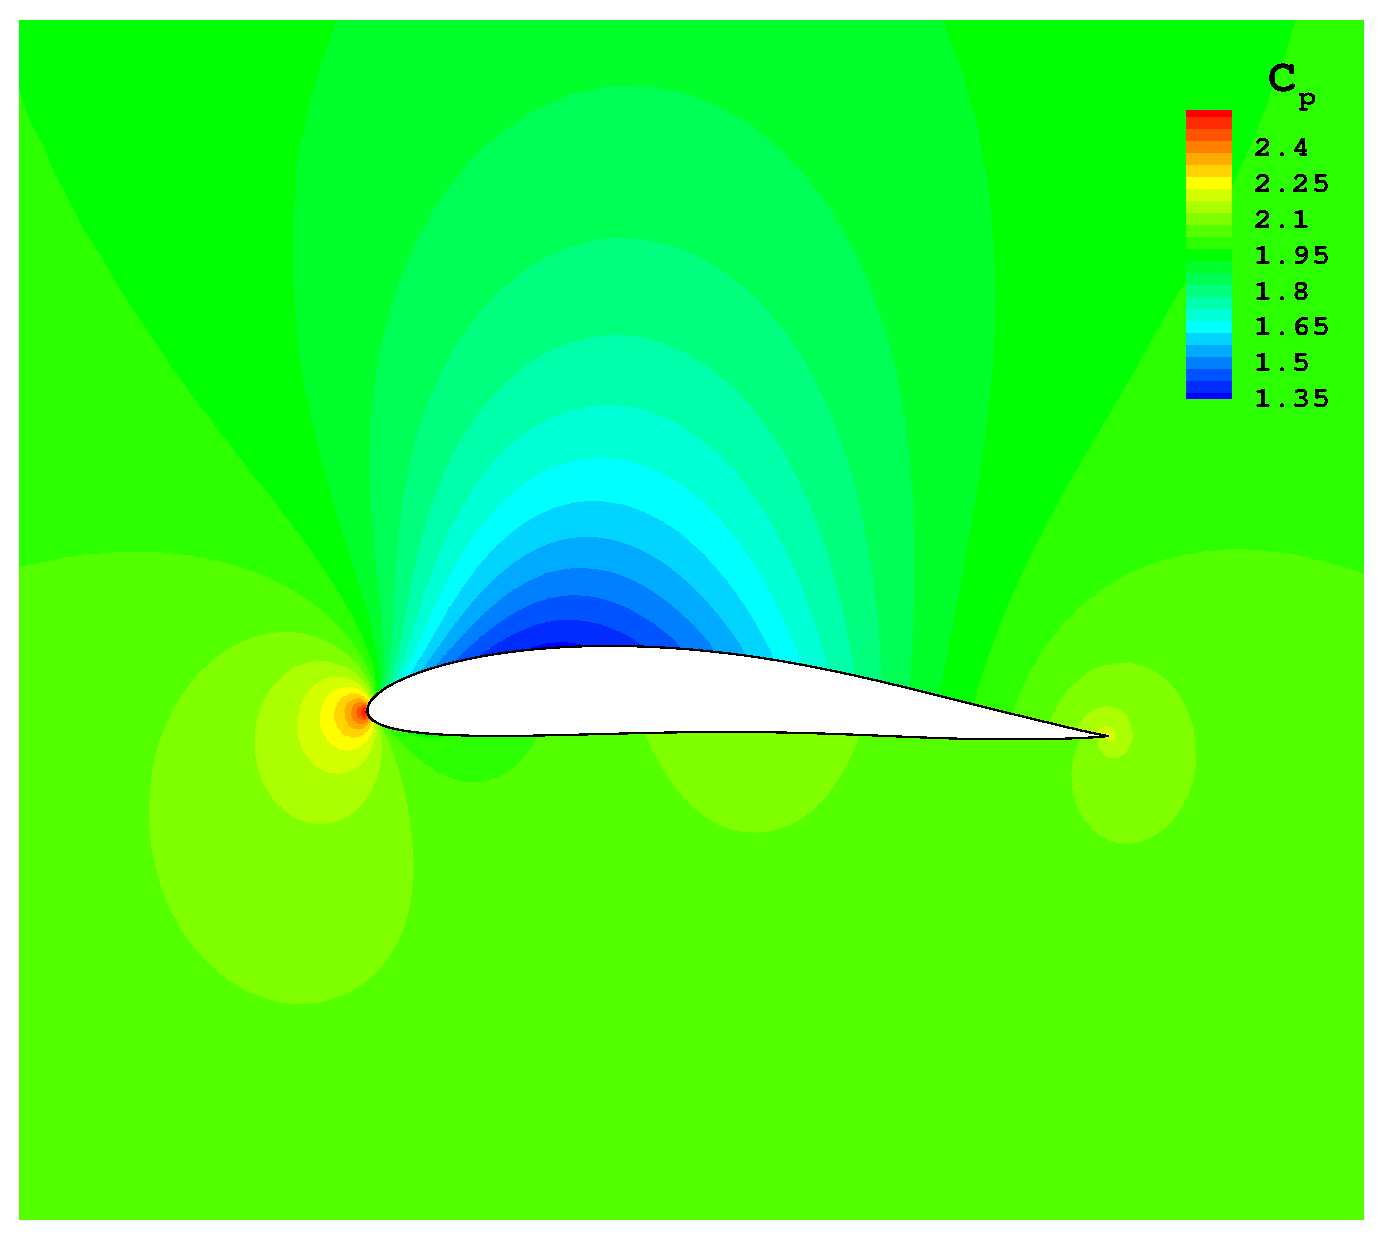
\includegraphics[width=1.0\textwidth]{RobustAirfoilKRk0.eps} \subcaption{Robust $k=0$}
  \end{minipage}
  \begin{minipage}[b]{0.30\linewidth}
    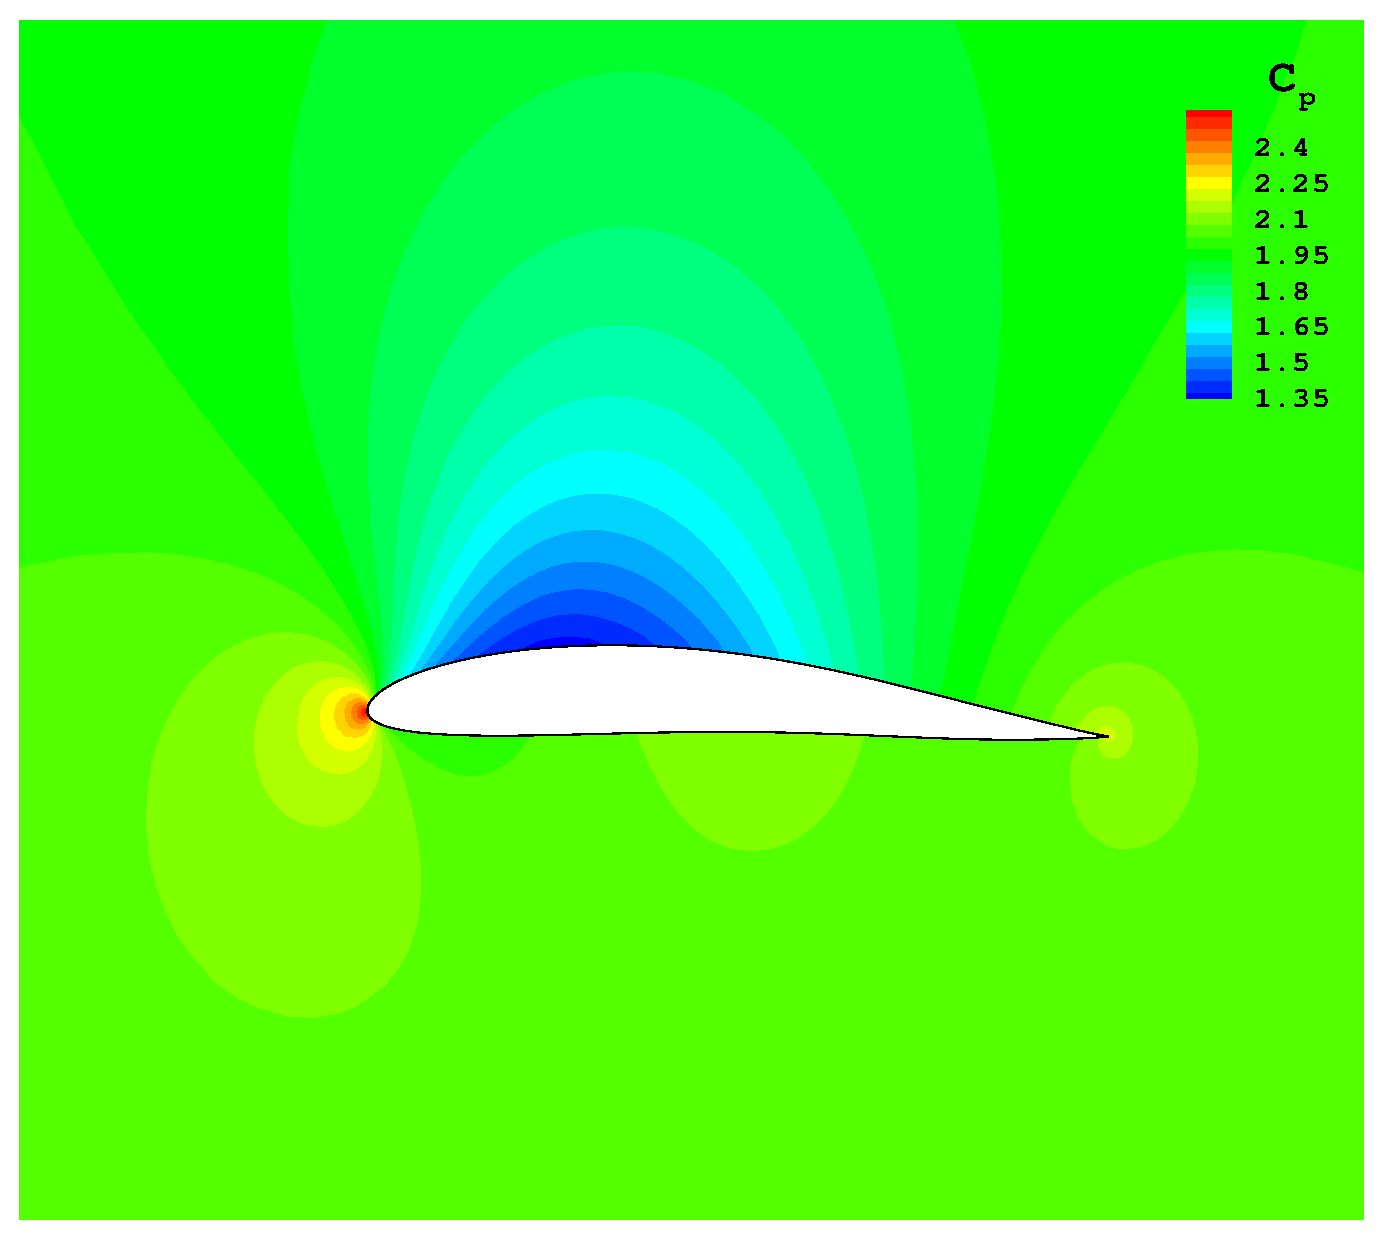
\includegraphics[width=1.0\textwidth]{RobustAirfoilKRk1.eps} \subcaption{Robust $k=1$}
  \end{minipage}
  \begin{minipage}[b]{0.30\linewidth}
    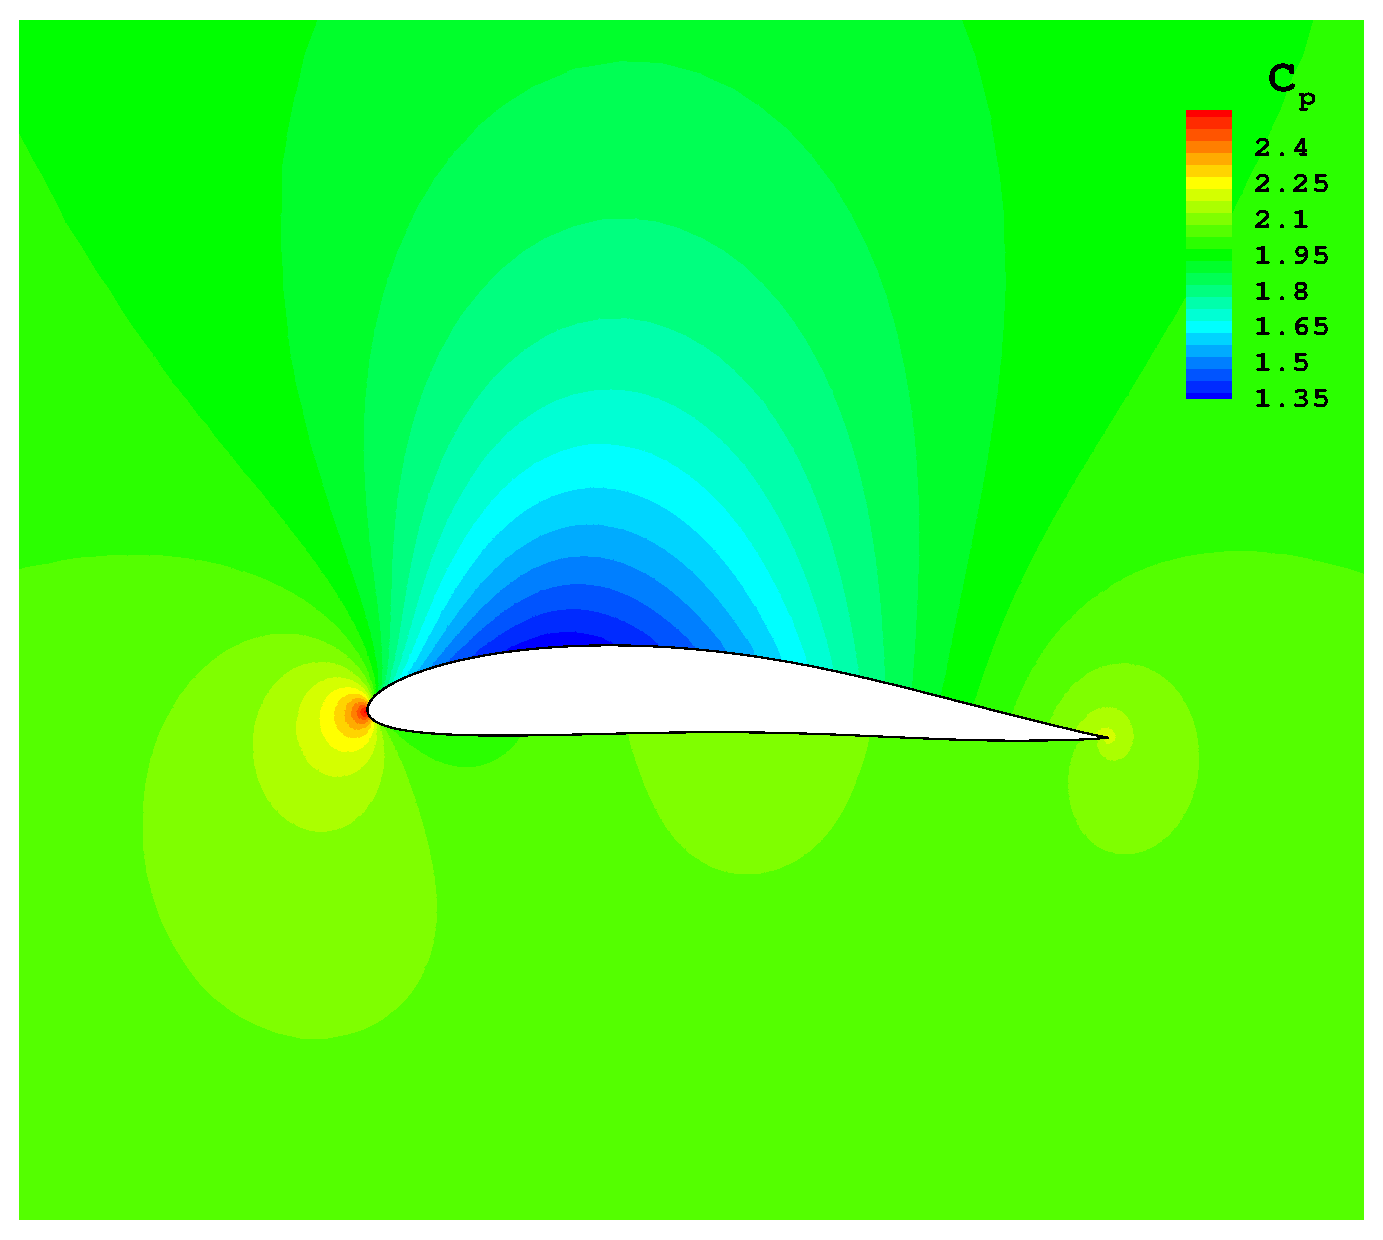
\includegraphics[width=1.0\textwidth]{RobustAirfoilKRk2.eps}\subcaption{Robust $k=2$}
  \end{minipage}
  \begin{minipage}[b]{0.30\linewidth}
    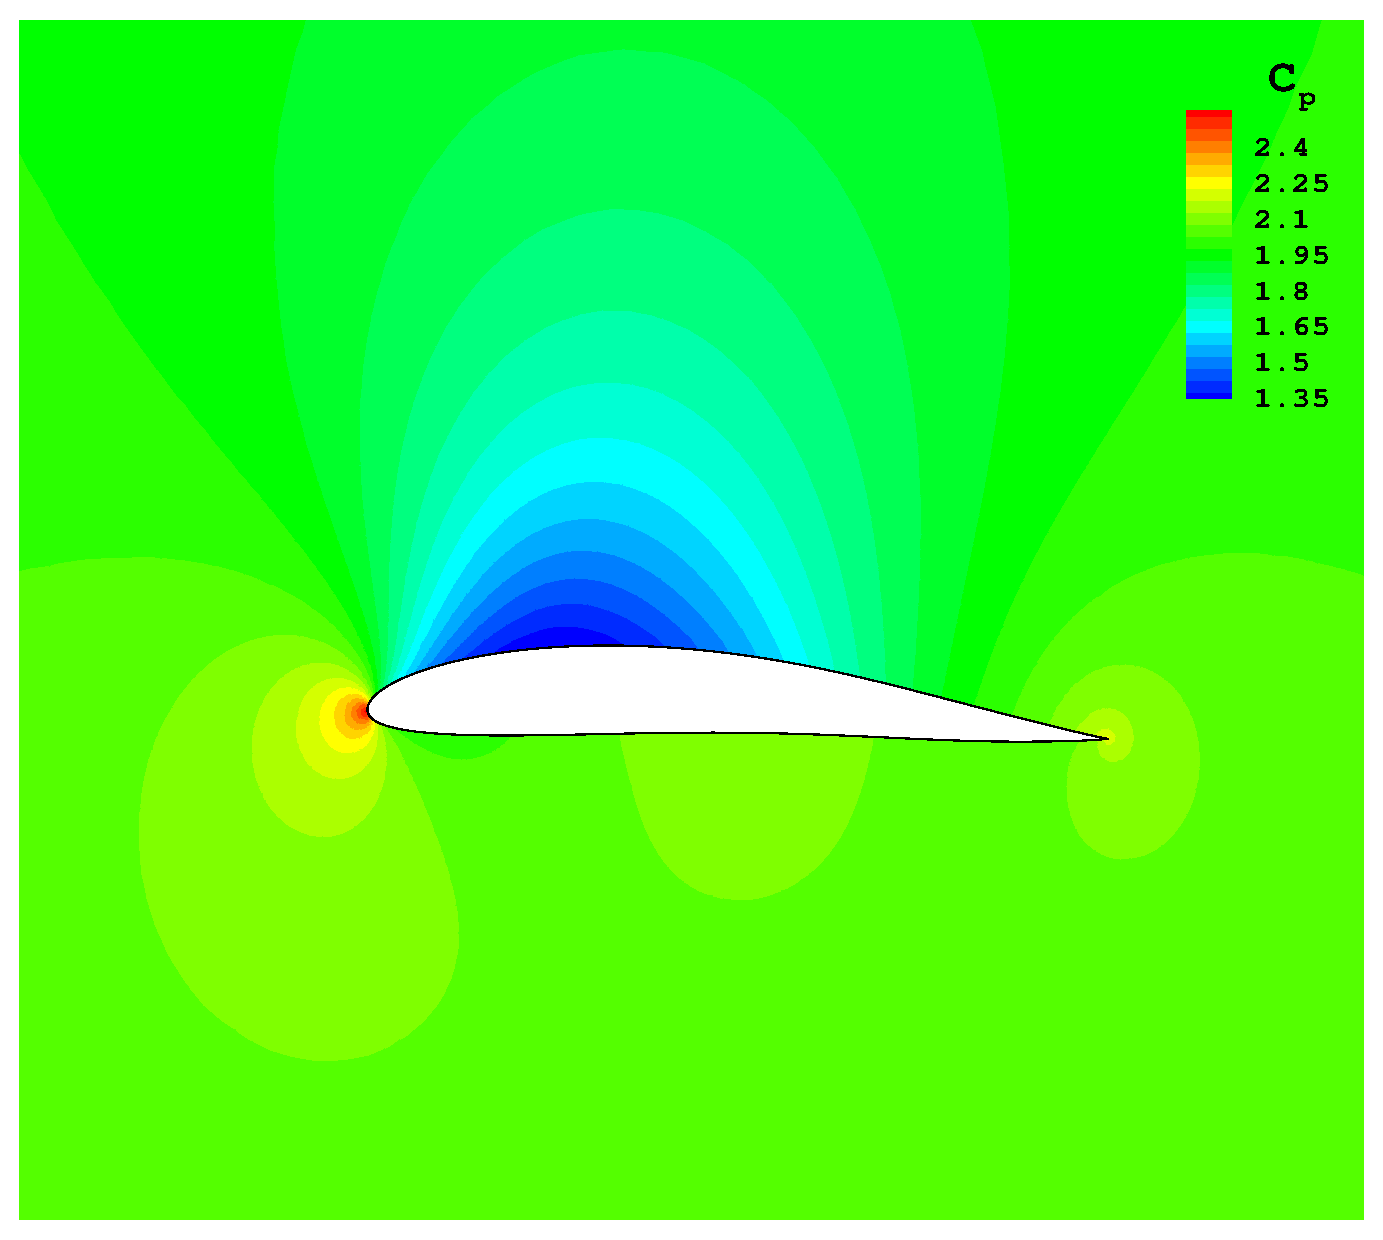
\includegraphics[width=1.0\textwidth]{RobustAirfoilKRk3.eps}\subcaption{Robust $k=3$}
  \end{minipage}
  \begin{minipage}[b]{0.30\linewidth}
    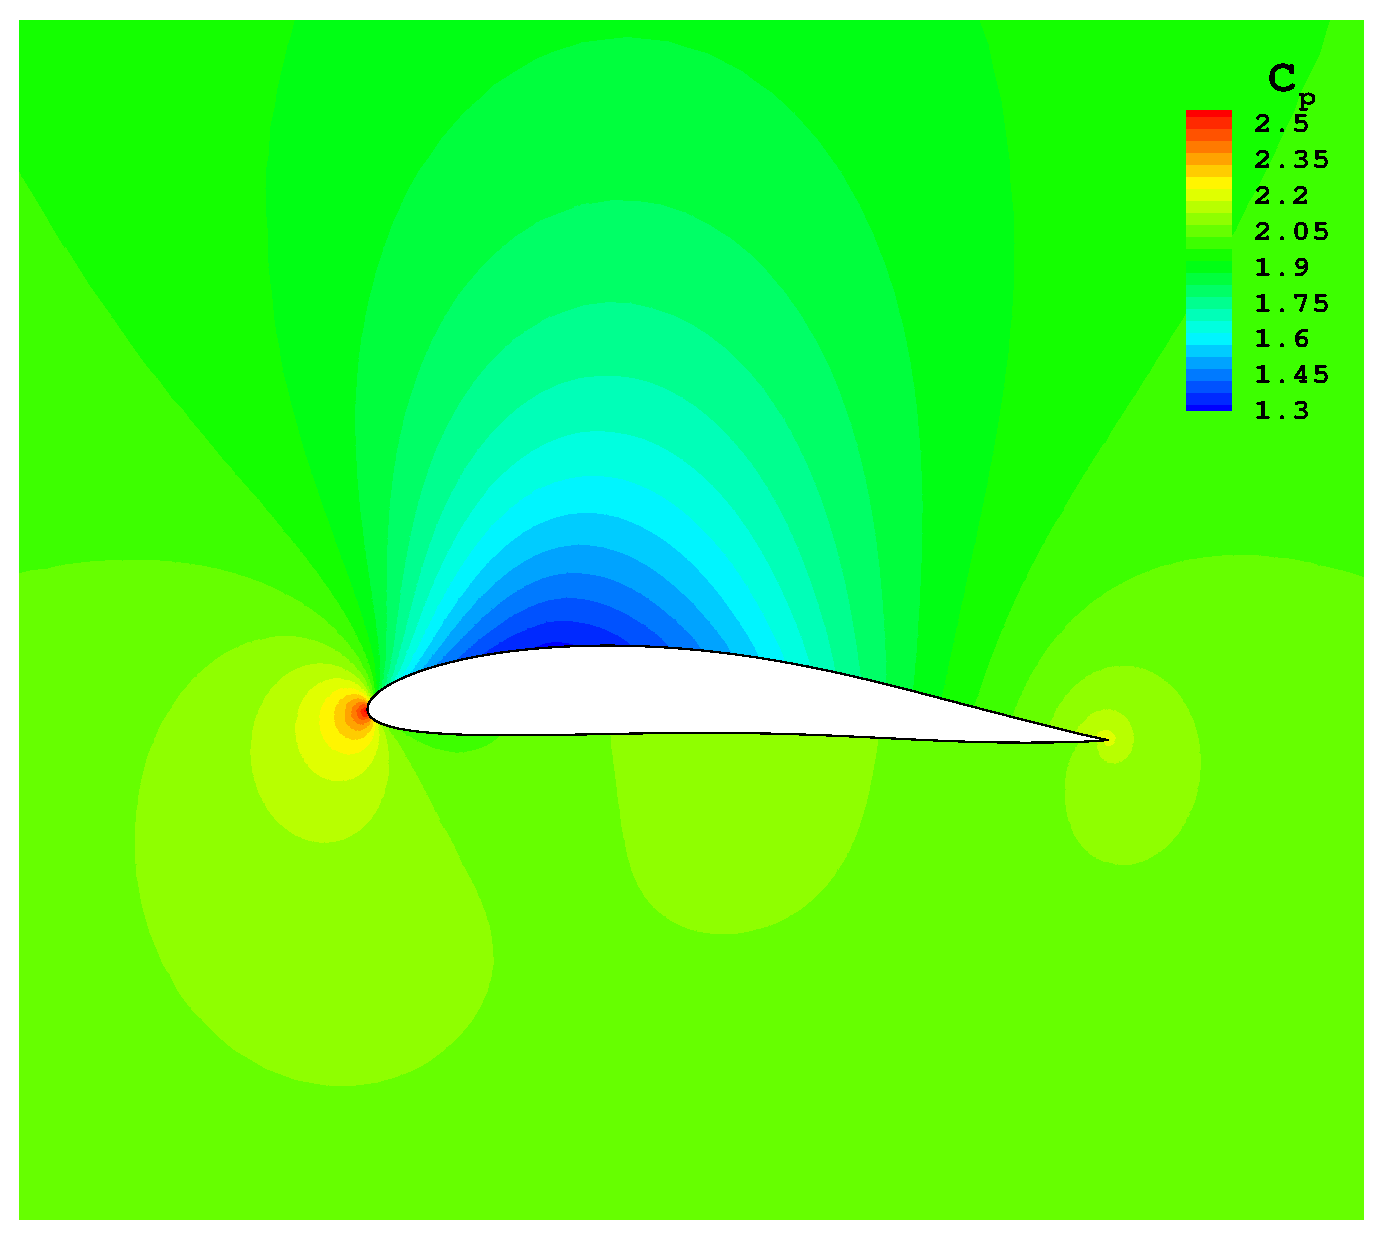
\includegraphics[width=1.0\textwidth]{RobustAirfoilKRk4.eps}\subcaption{Robust $k=4$}
  \end{minipage}
  \caption[Pressure contours around different airfoils produced using kriging.]{Contour plots of pressure coefficients $C_p$ at different optimum designs using kriging.}
  \label{CpContoursRobustKriging}
\end{figure}

\begin{figure}[h]
  \centering  
  \begin{minipage}[b]{0.30\linewidth}
    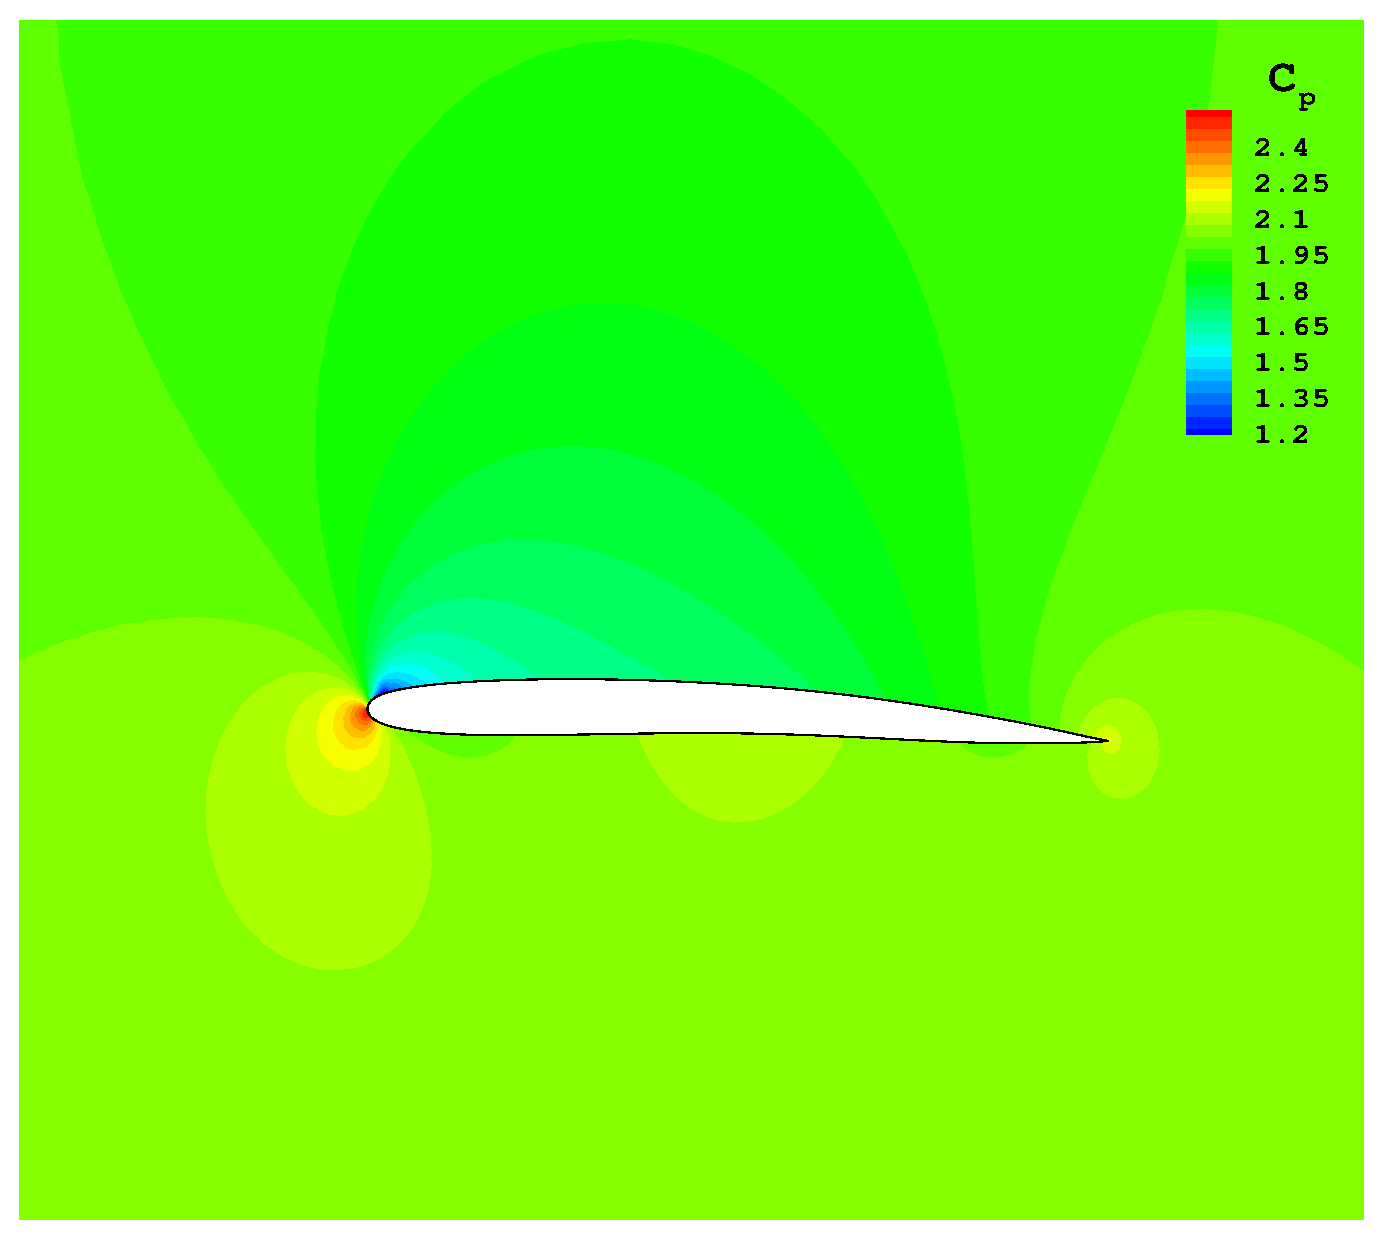
\includegraphics[width=1.0\textwidth]{DeterministicPressure.eps} \subcaption{Deterministic}
  \end{minipage}
  \begin{minipage}[b]{0.30\linewidth}
    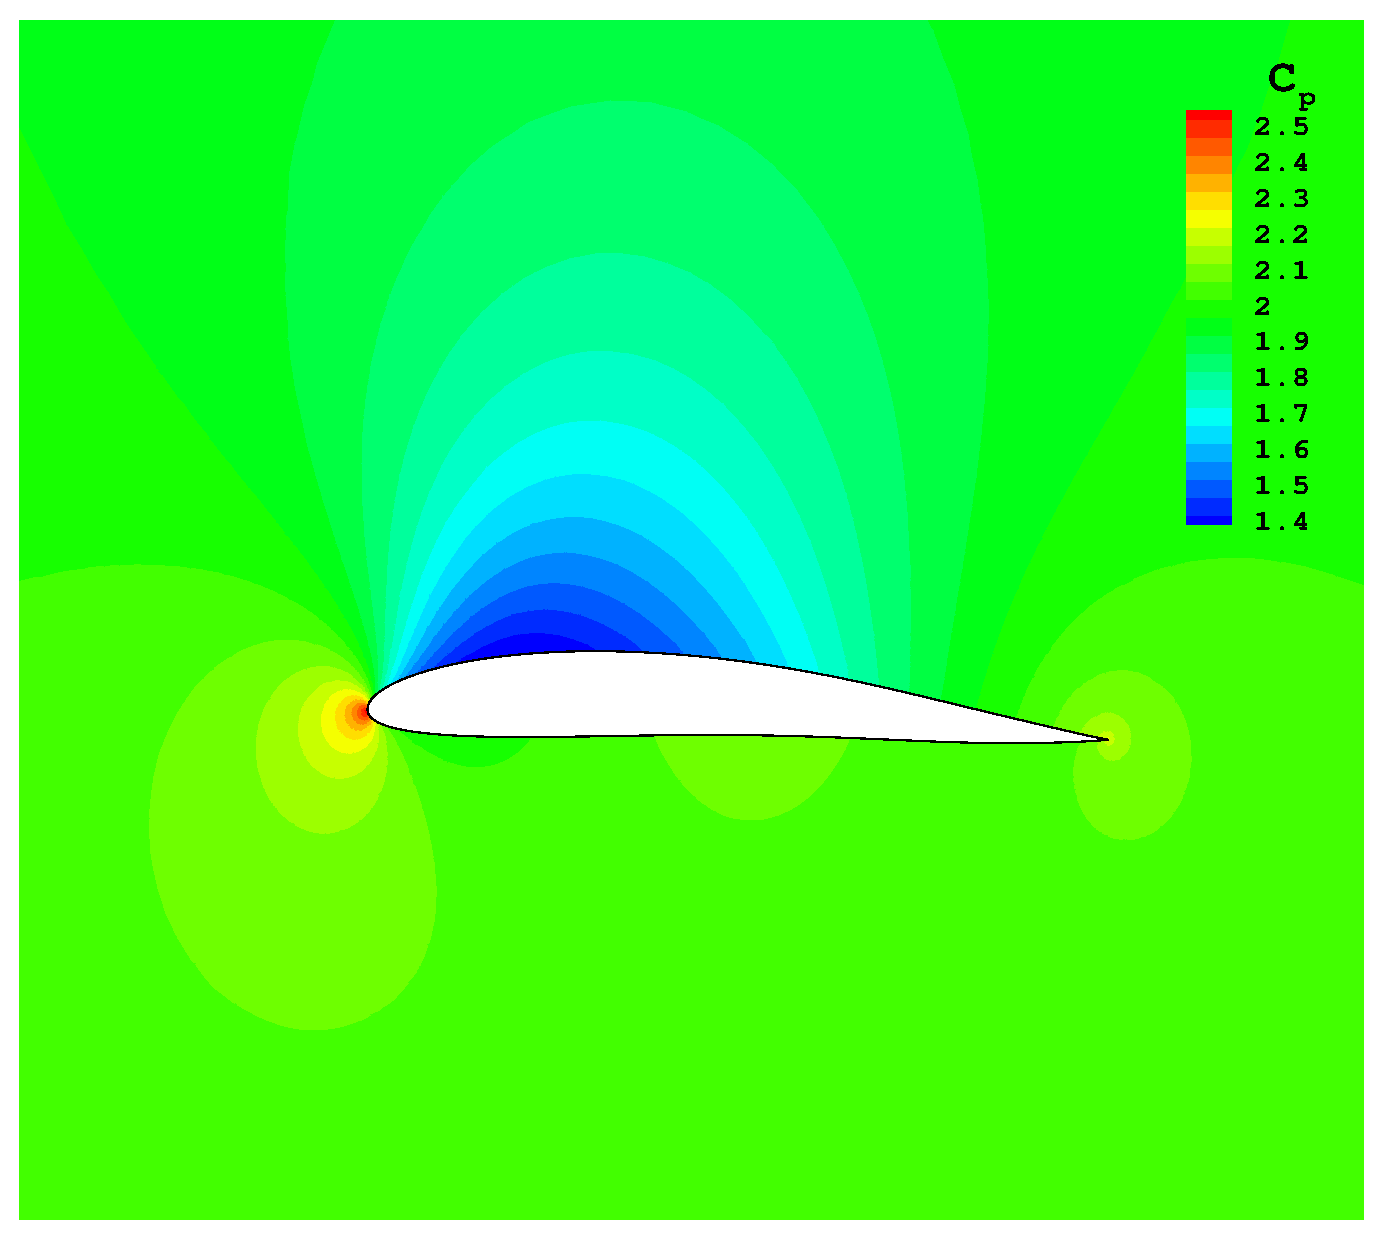
\includegraphics[width=1.0\textwidth]{RobustAirfoilPCk0.eps} \subcaption{Robust $k=0$}
  \end{minipage}
  \begin{minipage}[b]{0.30\linewidth}
    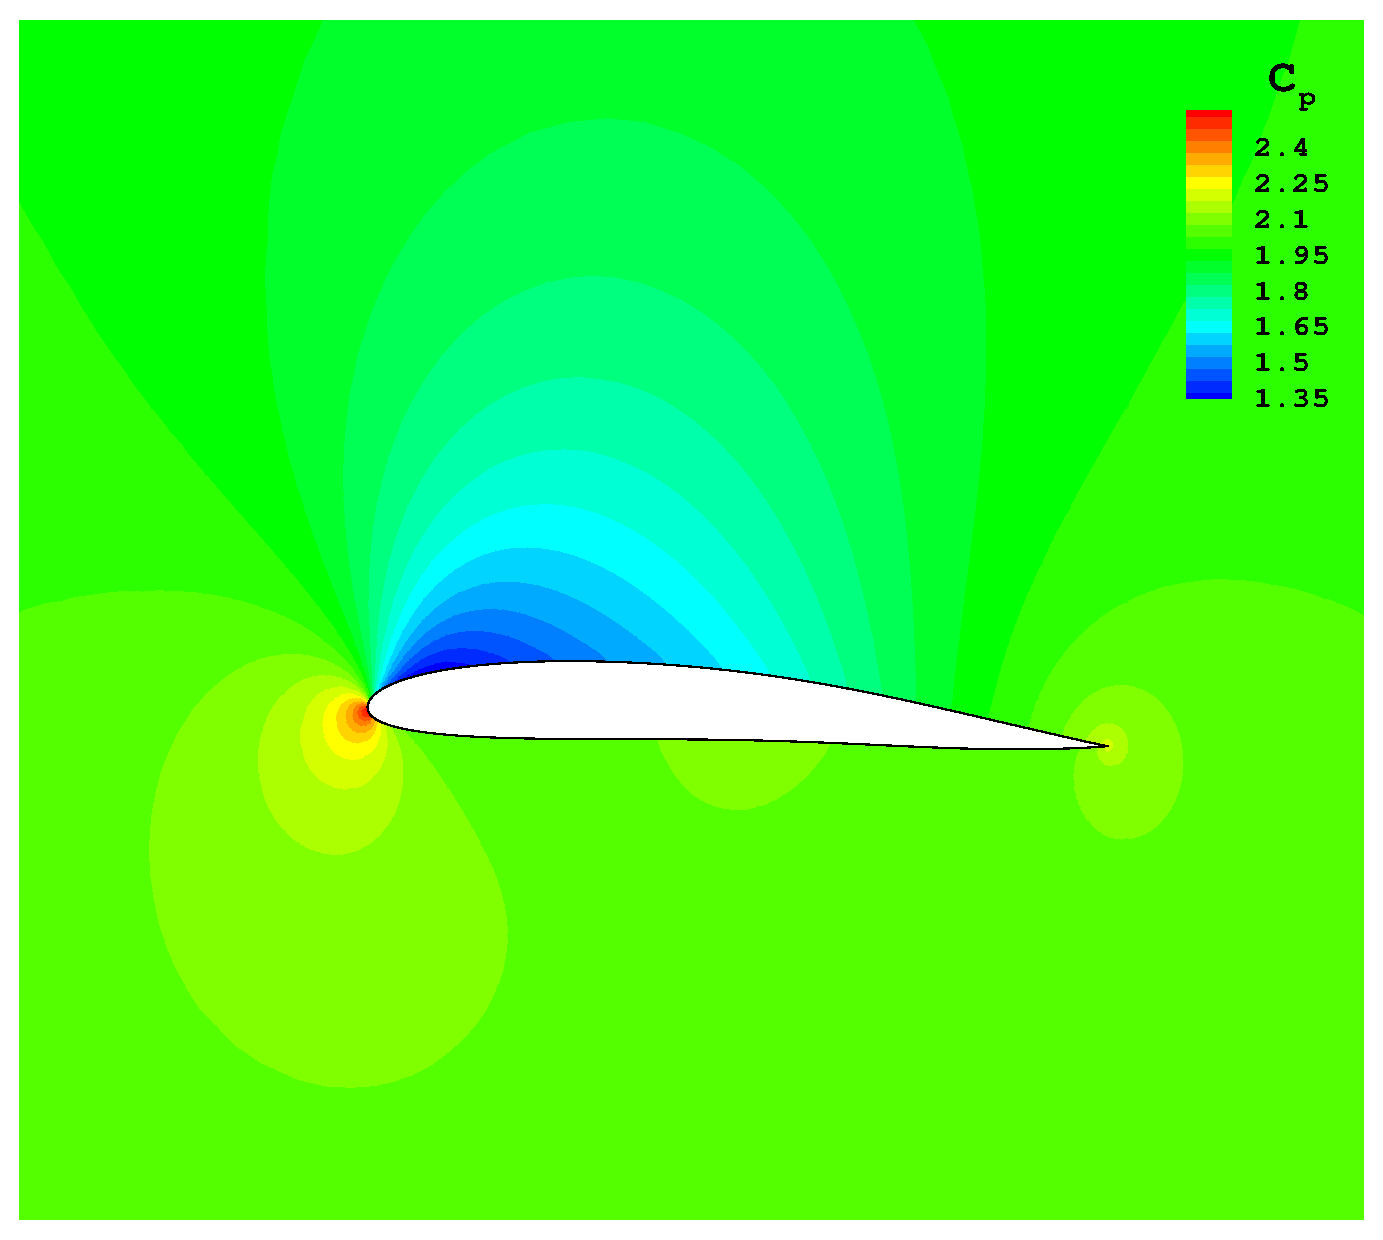
\includegraphics[width=1.0\textwidth]{RobustAirfoilPCk1.eps} \subcaption{Robust $k=1$}
  \end{minipage}
  \begin{minipage}[b]{0.30\linewidth}
    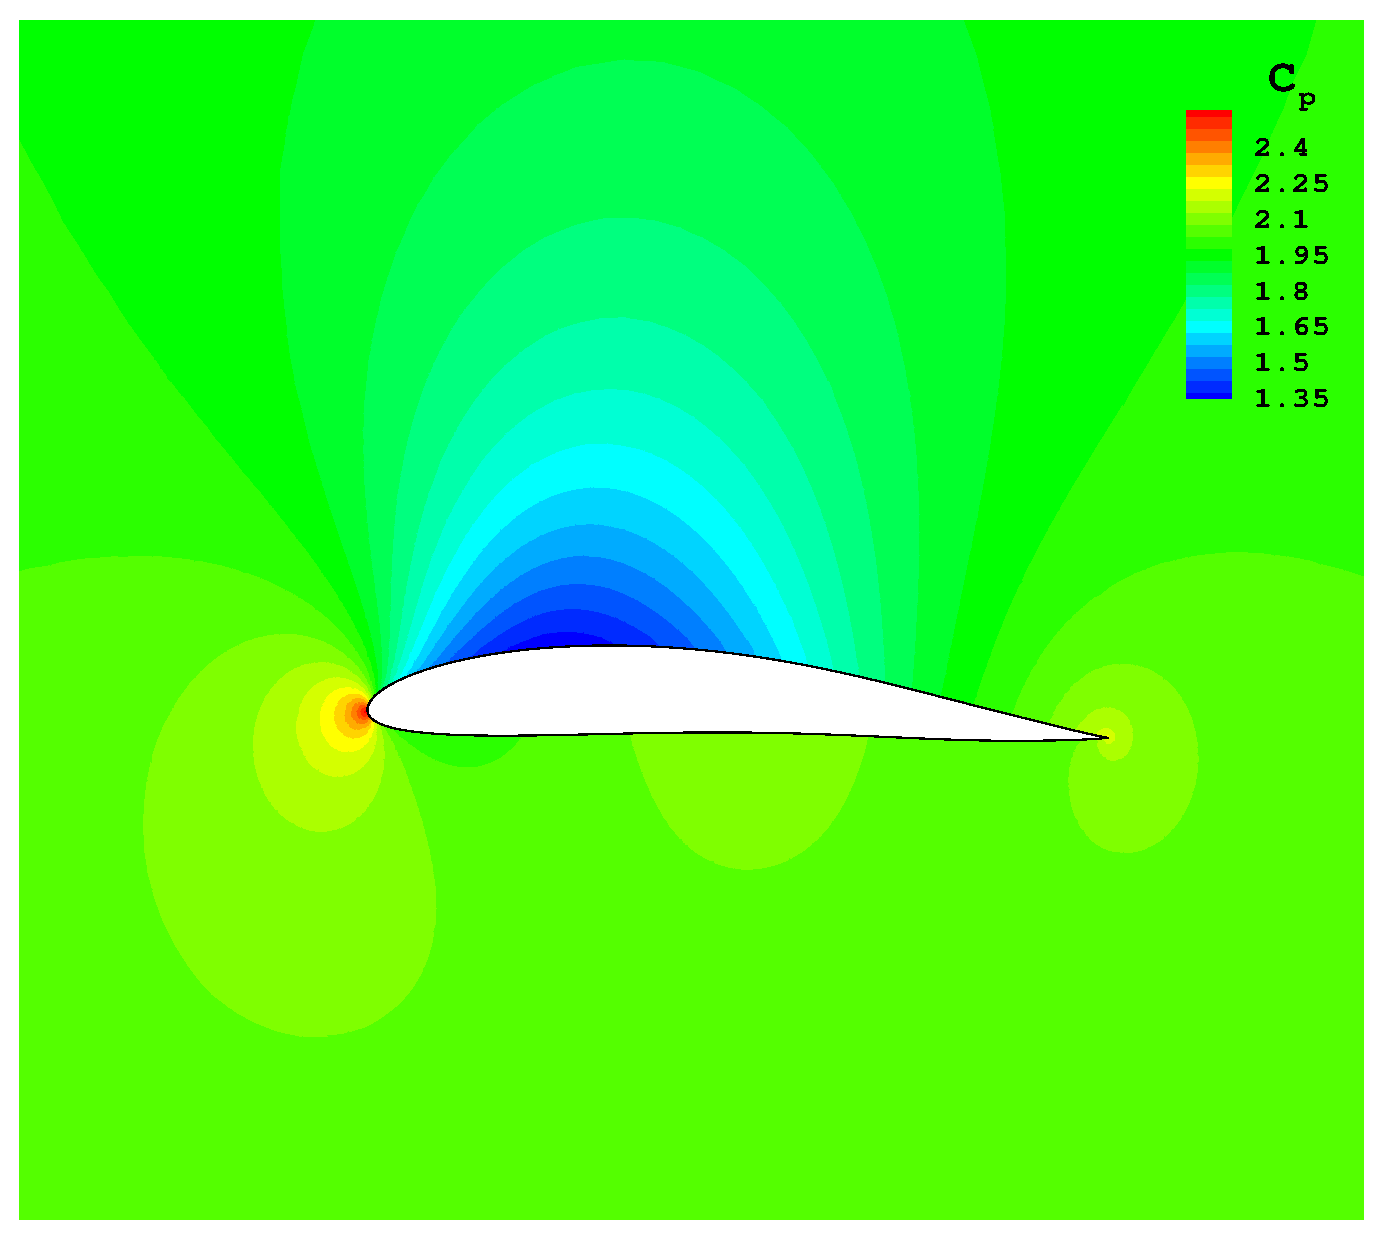
\includegraphics[width=1.0\textwidth]{RobustAirfoilPCk2.eps}\subcaption{Robust $k=2$}
  \end{minipage}
  \begin{minipage}[b]{0.30\linewidth}
    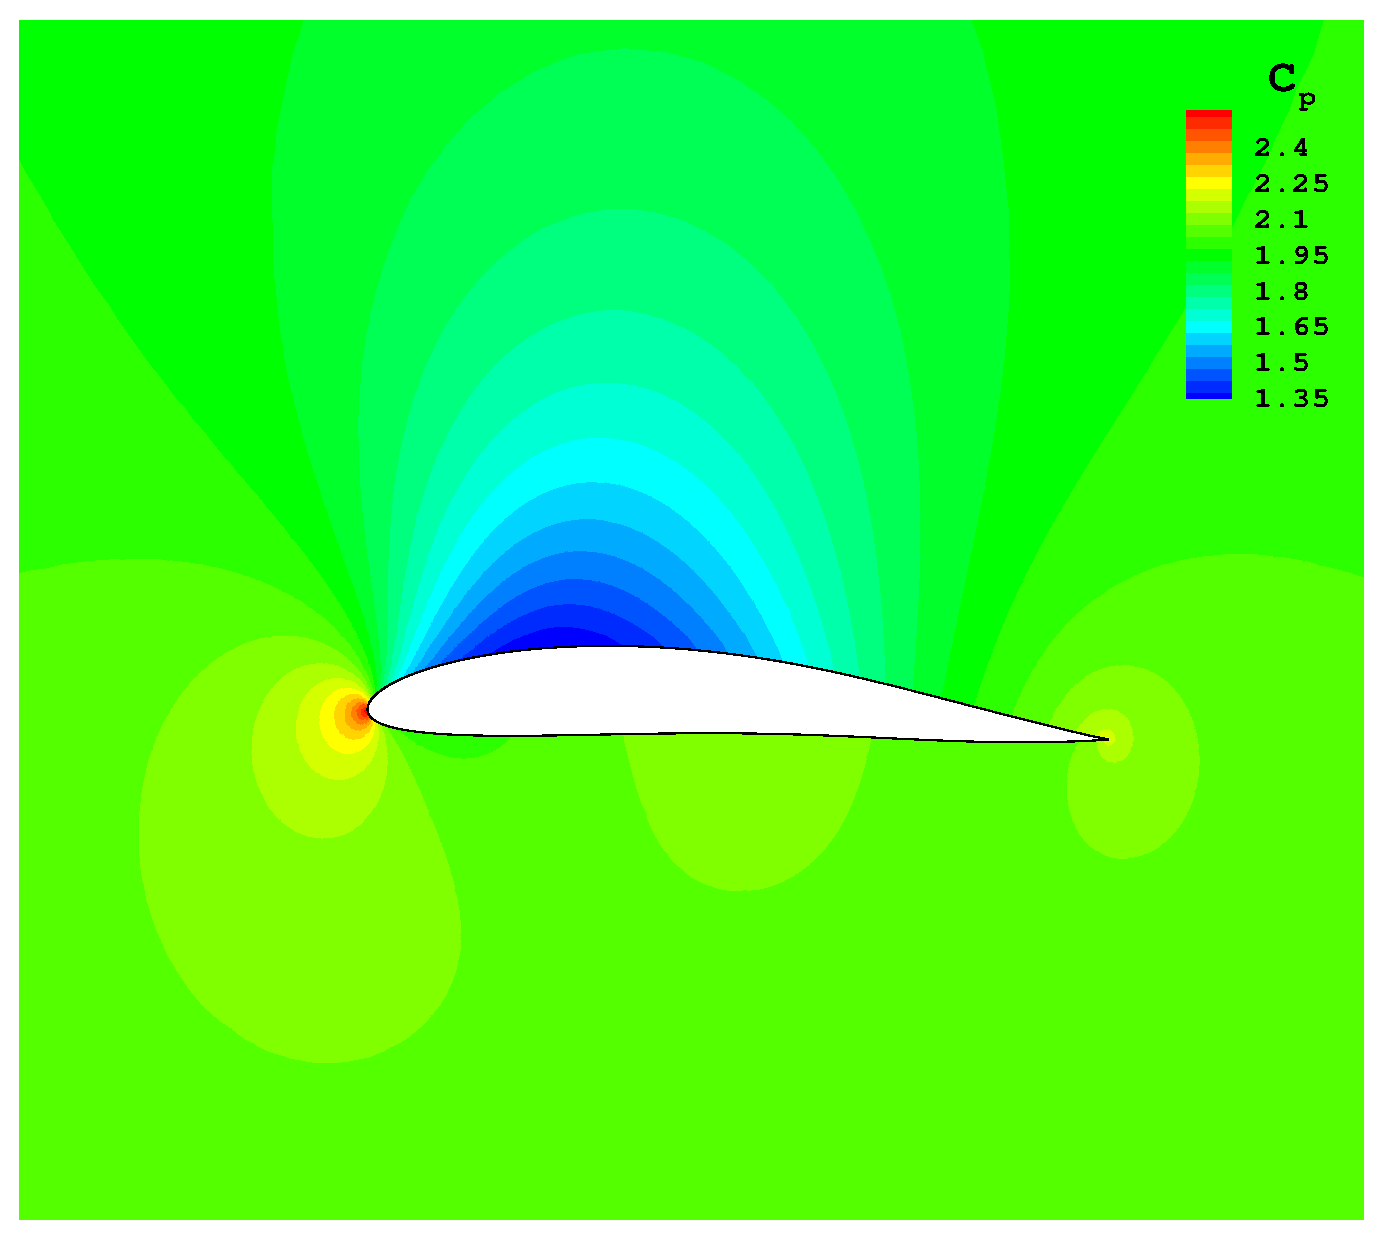
\includegraphics[width=1.0\textwidth]{RobustAirfoilPCk3.eps}\subcaption{Robust $k=3$}
  \end{minipage}
  \begin{minipage}[b]{0.30\linewidth}
    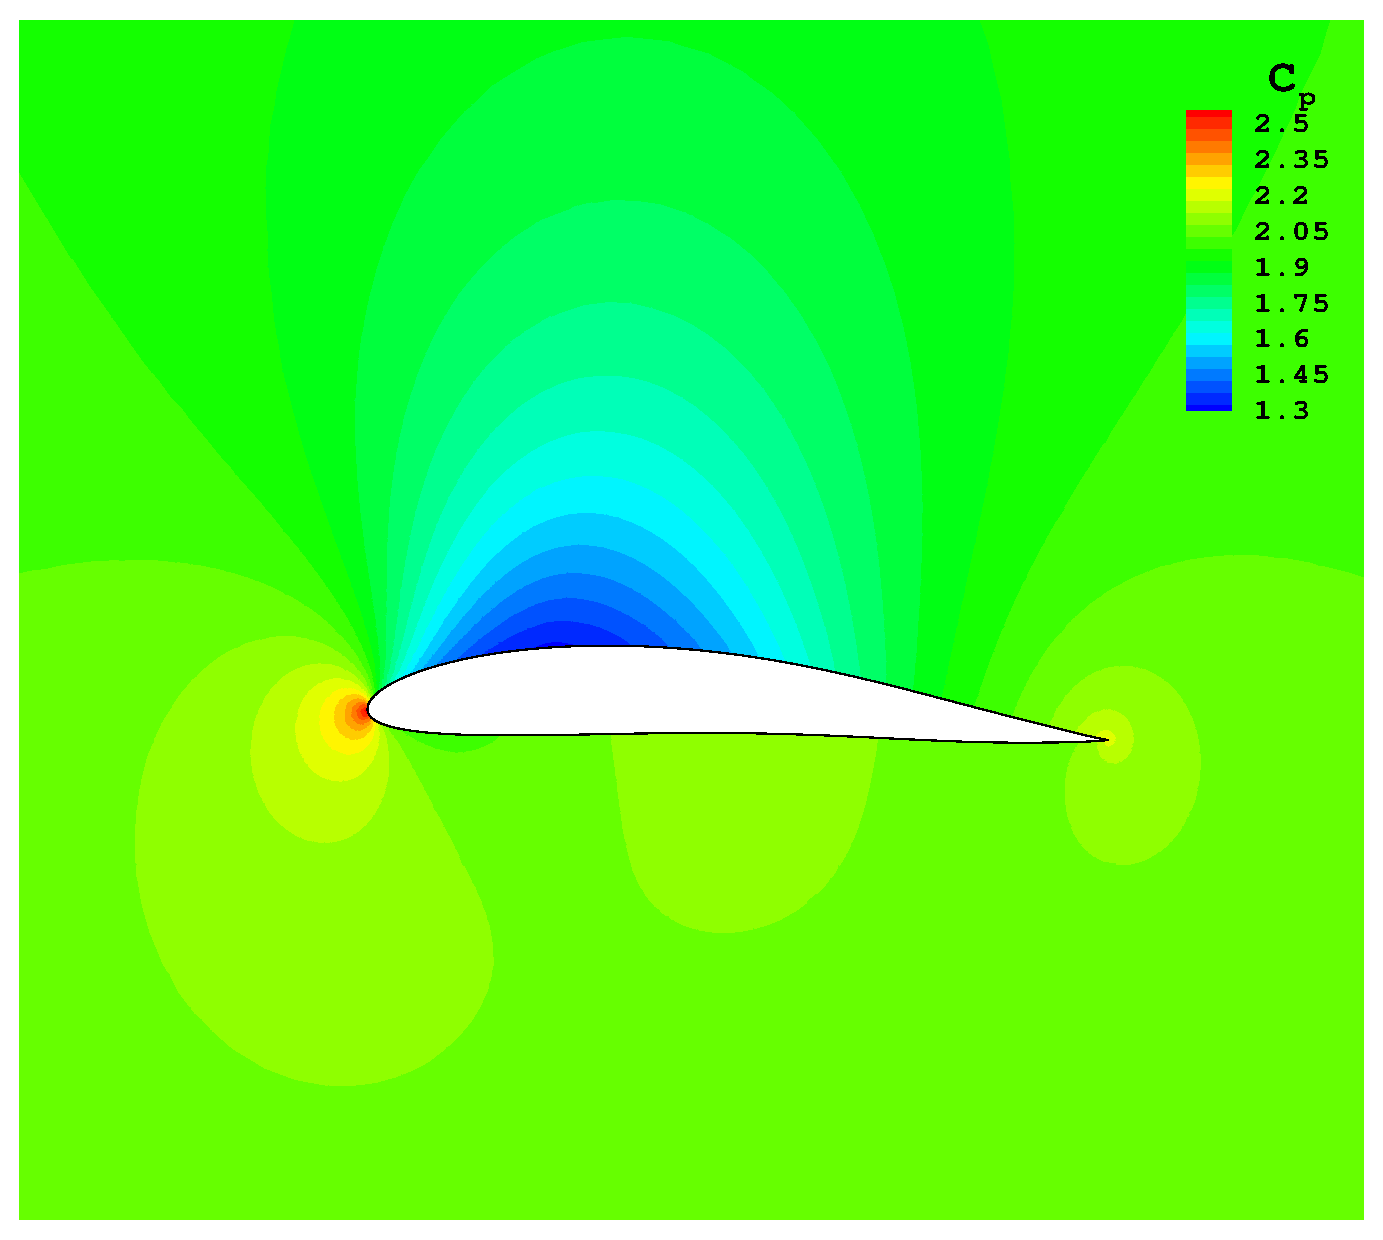
\includegraphics[width=1.0\textwidth]{RobustAirfoilPCk4.eps}\subcaption{Robust $k=4$}
  \end{minipage}
  \caption[Pressure contours around different airfoils produced using PCE.]{Contour plots of pressure coefficients $C_p$ at different optimum designs using PCE.}
  \label{CpContoursRobustPC}
\end{figure}


\subsection{Validation with Exact Monte Carlo Simulation}

Here, validations for the IMCS-BCO approach are provided by a selective comparison of the $k=1$ case with exact Monte Carlo simulation (MCS) and BCO ~\ie~the surrogate models are replaced with exact function evaluations (Euler flow solutions). 
Due to the expense of the Euler flow solutions, only $3000$ Monte Carlo samples are used for this test. For each Monte Carlo sample, a BCO problem is solved and statistics obtained are presented in Tables~\ref{initialvalid} and~\ref{finalvalid}.

\begin{table}[h!]
\caption[Selected validation of mixed uncertainty propagation at the initial design.]{Validations for $k=1$ robust case at the initial design (NACA 0012, $\alpha=2^{\circ}$ and $M_{\infty}=0.65$) for kriging and polynomial chaos.}
\medskip
\centering 
\scalebox{0.99}{\begin{tabular}{c|cc|cc|c}
\hline\hline
Type  &  $\mu_{{c}_{d_{max}}}$ & ${\sigma_{c_{d_{max}}}^2}$ & $\mu_{{c}_{l_{min}}}$ &  ${\sigma_{c_{l_{min}}}}$ & No. of Function/ \\
& & &  & & Gradient Evals.\\
\hline\hline
IMCS-BCO (Kriging) &  $8.85\cdot 10^{-4}$ & $4.32\cdot 10^{-9}$ & 0.186 & $1.72\cdot 10^{-2}$&  38/38 \\ 
IMCS-BCO (PC)      & $9.27\cdot 10^{-4}$ & $3.97\cdot 10^{-8}$ & 0.186 & $1.72\cdot 10^{-2}$ & 36/36 \\
\hline
MCS-BCO  &  $8.98\cdot 10^{-4}$ & $2.98\cdot 10^{-8}$ & 0.186 & $1.72\cdot 10^{-2}$&  6153/6153 \\
\hline
\end{tabular}}
\label{initialvalid}
\end{table}

\begin{table}[h!]
\caption[Selected validation of mixed uncertainty propagation at the final design.]{Validations  for $k=1$ robust case at the final design for kriging (robust shape, $\alpha=2.065^{\circ}$ and $M_{\infty}=0.6$) and polynomial chaos (robust shape, $\alpha=3.058^{\circ}$ and $M_{\infty}=0.6$).}
\medskip
\centering 
\scalebox{0.99}{\begin{tabular}{c|cc|cc|c}
\hline\hline
Type  &  $\mu_{{c}_{d_{max}}}$ & ${\sigma_{c_{d_{max}}}^2}$ & $\mu_{{c}_{l_{min}}}$ &  ${\sigma_{c_{l_{min}}}}$ & No. of Function /\\
& & &  & & Gradient Evals.\\
\hline\hline
IMCS-BCO (Kriging) & $2.93\cdot 10^{-3}$ & $3.07\cdot 10^{-7}$ & $0.619$ & $1.86\cdot 10^{-2}$ & 23/23 \\
MCS-BCO     & $2.73\cdot 10^{-3}$ & $2.50\cdot 10^{-7}$ & $0.618$ & $1.84\cdot 10^{-2}$ & 23/23 \\
\hline
IMCS-BCO (PC)    & $2.96\cdot 10^{-3}$  & $2.86\cdot 10^{-7}$ & $0.619$  & $1.86\cdot 10^{-2}$ & 6153/6153 \\
MCS-BCO    & $2.65\cdot 10^{-3}$ & $2.90\cdot 10^{-8}$ & $0.620$ & $1.81\cdot10^{-2}$& 6152/6152 \\
\hline
\end{tabular}}
\label{finalvalid}
\end{table}

Overall, it can be noticed that the surrogate models produce reasonably accurate statistics for a fraction of the computational cost compared to MCS. Also, kriging is more accurate than polynomial chaos in predicting the statistics.



